\documentclass[]{agujournal2019}
\usepackage{url} %this package should fix any errors with URLs in refs.
\usepackage{lineno}
\usepackage[inline]{trackchanges} %for better track changes. finalnew option will compile document with changes incorporated.
\usepackage{soul}
\usepackage{amsmath}
%\linenumbers

\draftfalse

\journalname{JGR: Solid Earth}

\begin{document}

\title{Bayesian paleomagnetic Euler pole inversion for paleogeographic reconstruction and analysis}

\authors{Ian R. Rose\affil{1}, Yiming Zhang\affil{1}, and Nicholas L. Swanson-Hysell\affil{1}}


 \affiliation{1}{Department of Earth and Planetary Science, University of California, Berkeley, CA, USA}

\correspondingauthor{Nicholas L. Swanson-Hysell}{swanson-hysell@berkeley.edu}

\vspace{0.5 in}
\noindent This paper was published as:

\noindent Rose, I. R., Zhang, Y., and Swanson-Hysell, N. L. (2022). Bayesian paleomagnetic Euler pole inversion for paleogeographic reconstruction and analysis. Journal  Geophysical Research: Solid Earth, 127, e2021JB023890. https://doi.org/10.1029/2021JB023890

\begin{keypoints}
\item Paleomagnetic Euler pole analysis can be implemented as a Bayesian inverse problem that incorporates uncertainty on pole positions and ages
\item This approach provides estimates of absolute plate rates with uncertainties and can solve for the timing of Euler pole changepoints
\item Applying this method to Australia paleomagnetic data yields plate motions that are consistent with those from independent plate models
\end{keypoints}

\begin{abstract}
Apparent polar wander paths (APWPs) synthesized from paleomagnetic poles provide the most direct data for reconstructing past paleogeography and plate motions for times earlier than ca. 200 Ma. In this contribution, we describe a new method for APWP synthesis that extends the paleomagnetic Euler pole analysis of \citeA{Gordon1984a} by placing it within the framework of a Bayesian inverse problem. This approach incorporates uncertainties in pole positions and age that are often ignored in standard treatments. The paleomagnetic Euler poles resulting from the inversions provide estimates for full-vector plate motion (both latitude and longitude) and associated uncertainty. The method allows for inverting for one or more Euler poles with the timing of changepoints being solved as part of the inversion. In addition, the method allows the incorporation of true polar wander rotations, thus providing an avenue for probabilistic partitioning of plate tectonic motion and true polar wander based on paleomagnetic poles. We show example inversions on synthetic data to demonstrate the method's capabilities. We illustrate application of the method to Cenozoic Australia paleomagnetic poles which can be compared to independent plate reconstructions. A two-Euler pole inversion for the Australian record recovers northward acceleration of Australia in the Eocene with rates that are consistent with plate reconstructions. We also apply the method to constrain rapid rates of motion for cratonic North America associated with the Keweenawan Track of late Mesoproterozoic paleomagnetic poles. The application of Markov chain Monte Carlo methods to estimate paleomagnetic Euler poles can open new directions in quantitative paleogeography.
\end{abstract}

\section*{Plain Language Summary}
Movement of Earth's tectonic plates results in large changes in continent positions over time known as paleogeography. Reconstructing paleogeography is central for understanding long term changes to Earth's surface and interior. Ocean floor data are very useful for determining these motions, but only exist for the most recent 4$\%$ of Earth's history. For older times, we use magnetic directions in rocks that show positions relative to the north pole. These records are called paleomagnetic poles and plate motions result in progressions of paleomagnetic poles called paths. Earth scientists need ways to synthesize poles into paths. Ideally, such a synthesis uses uncertainties on pole positions and ages. We developed a new way to reconstruct plate motion from paleomagnetic poles using an approach called Bayesian inversion. We apply the method to pretend data to illustrate its capabilities. We then apply the method to real data such as that from Australia over the past 60 million years. This analysis shows change in the continent's position and the rate of its motion that is similar to approaches that rely on ocean floor data. For older times, the method can help reconstruct positions and provide estimates of plate motion rates and associated uncertainty. 


\section{Introduction}

Plate tectonics is the differential motion of near-rigid blocks of lithosphere across the surface of Earth, separated by relatively narrow regions of deformation in spreading centers, transform faults, and subduction zones. The relative rigidity of plates means that the motion of most of Earth's surface can be described by a set of Euler poles which specify the position (in latitude and longitude) of a rotation axis and a rate of rotation about this axis for a given plate \cite<cf.>{Cox2009a}. Individual points on a plate undergoing rigid rotation are described by small circle paths (Fig. \ref{fig:pep}).

Euler poles are widely used for describing plate motions due to their simplicity and compactness \cite<e.g.>{DeMets2010a, Argus2011a}. Motion between tectonic plates has a tendency to remain constant, or approximately so, over time scales of millions of years \cite<e.g.>{Iaffaldano2012a, Muller2016a}. This consistency of motion can be seen physically expressed in the shape of oceanic fracture zones and in hotspot tracks across the lithosphere. These features often form gently curving arcs over large portions of Earth's surface that can be well described by small circles, consistent with finite Euler rotations of the plate for an extended period of time. As such, the combination of an Euler pole plus a time interval for which it is active (often called a ``stage pole'') is a convenient description of plate motions through Earth history.

The stage pole description of plate motions has been widely used in both continental reconstructions \cite<e.g.>{Boyden2011a} and in geodynamical modeling \cite<e.g.>{Mcnamara2005a, Bull2014a}. Most reconstructions of plate motions over the past 200 million years rely heavily on fitting Euler pole rotations to oceanic fracture zones, hotspot tracks, seafloor magnetic isochrons, and, to a lesser extent, paleomagnetic data \cite{Muller1993a, Seton2012a, Muller2016a}. These relative plate motions are used to construct plate circuits that relate plates to one another and to the spin axis \cite<e.g.>{Muller2016a, Torsvik2017a}. However, as we look further back in Earth history, many of the records on which these plate tectonic reconstructions rely largely disappear due to the subduction of oceanic lithosphere. Given the lack of oceanic crust older than $\sim$200 Ma, the paleomagnetic record from continental rocks is the dominant remaining data. These paleomagnetic data can be used in conjunction with geological data that provides information on the tectonic setting of continental margins as well as additional information, such as the correlation of geologic terranes, to develop paleogeographic reconstructions.

It is more challenging to reconstruct past plate motions from paleomagnetic pole positions than from data derived from oceanic lithosphere for a number of reasons, including: (1) the data are often sparser; (2) traditional paleomagnetic analysis constrains paleolatitude and the orientation of a continental block, but does not constrain paleolongitude without additional assumptions; and (3) paleomagnetic poles can have appreciable uncertainty in both position and age.

\citeA{Gordon1984a} noted that progressions of paleomagnetic poles (which are commonly referred to as apparent polar wander paths; APWPs) have arcing trajectories similar to fracture zones and hotspot tracks. This similar geometry is expected given that they are also tracking plate motion (Fig. \ref{fig:pep}). Building on the approach of \citeA{Francheteau1969a}, \citeA{Gordon1984a} developed an algorithm to find the best-fit small circles to paleomagnetic poles, which would furnish Euler poles for the plate in question for that time period. This approach for constraining APWPs, called paleomagnetic Euler pole analysis, has the attractive feature of providing a complete description of the plate motion, including paleolongitudinal changes and therefore rates of motion. However, it has the drawback of not providing readily computed uncertainties associated with the paleomagnetic poles and not incorporating age uncertainties. An additional complexity is that while relative motions between tectonic plates can be consistent over extended periods and explained by a single Euler, absolute plate motion relative to the spin axis can be more time variable due to changes associated with one of multiple Euler rotations through a plate circuit or due to a combination of plate tectonic motion and true polar wander. With some notable exceptions \cite<e.g.>{Bryan1986a, Beck1989a, Tarling1996a, Beck2003a, Smirnov2010a}, paleomagnetic Euler pole analysis has not seen wide adoption. 

\begin{figure}
\centering
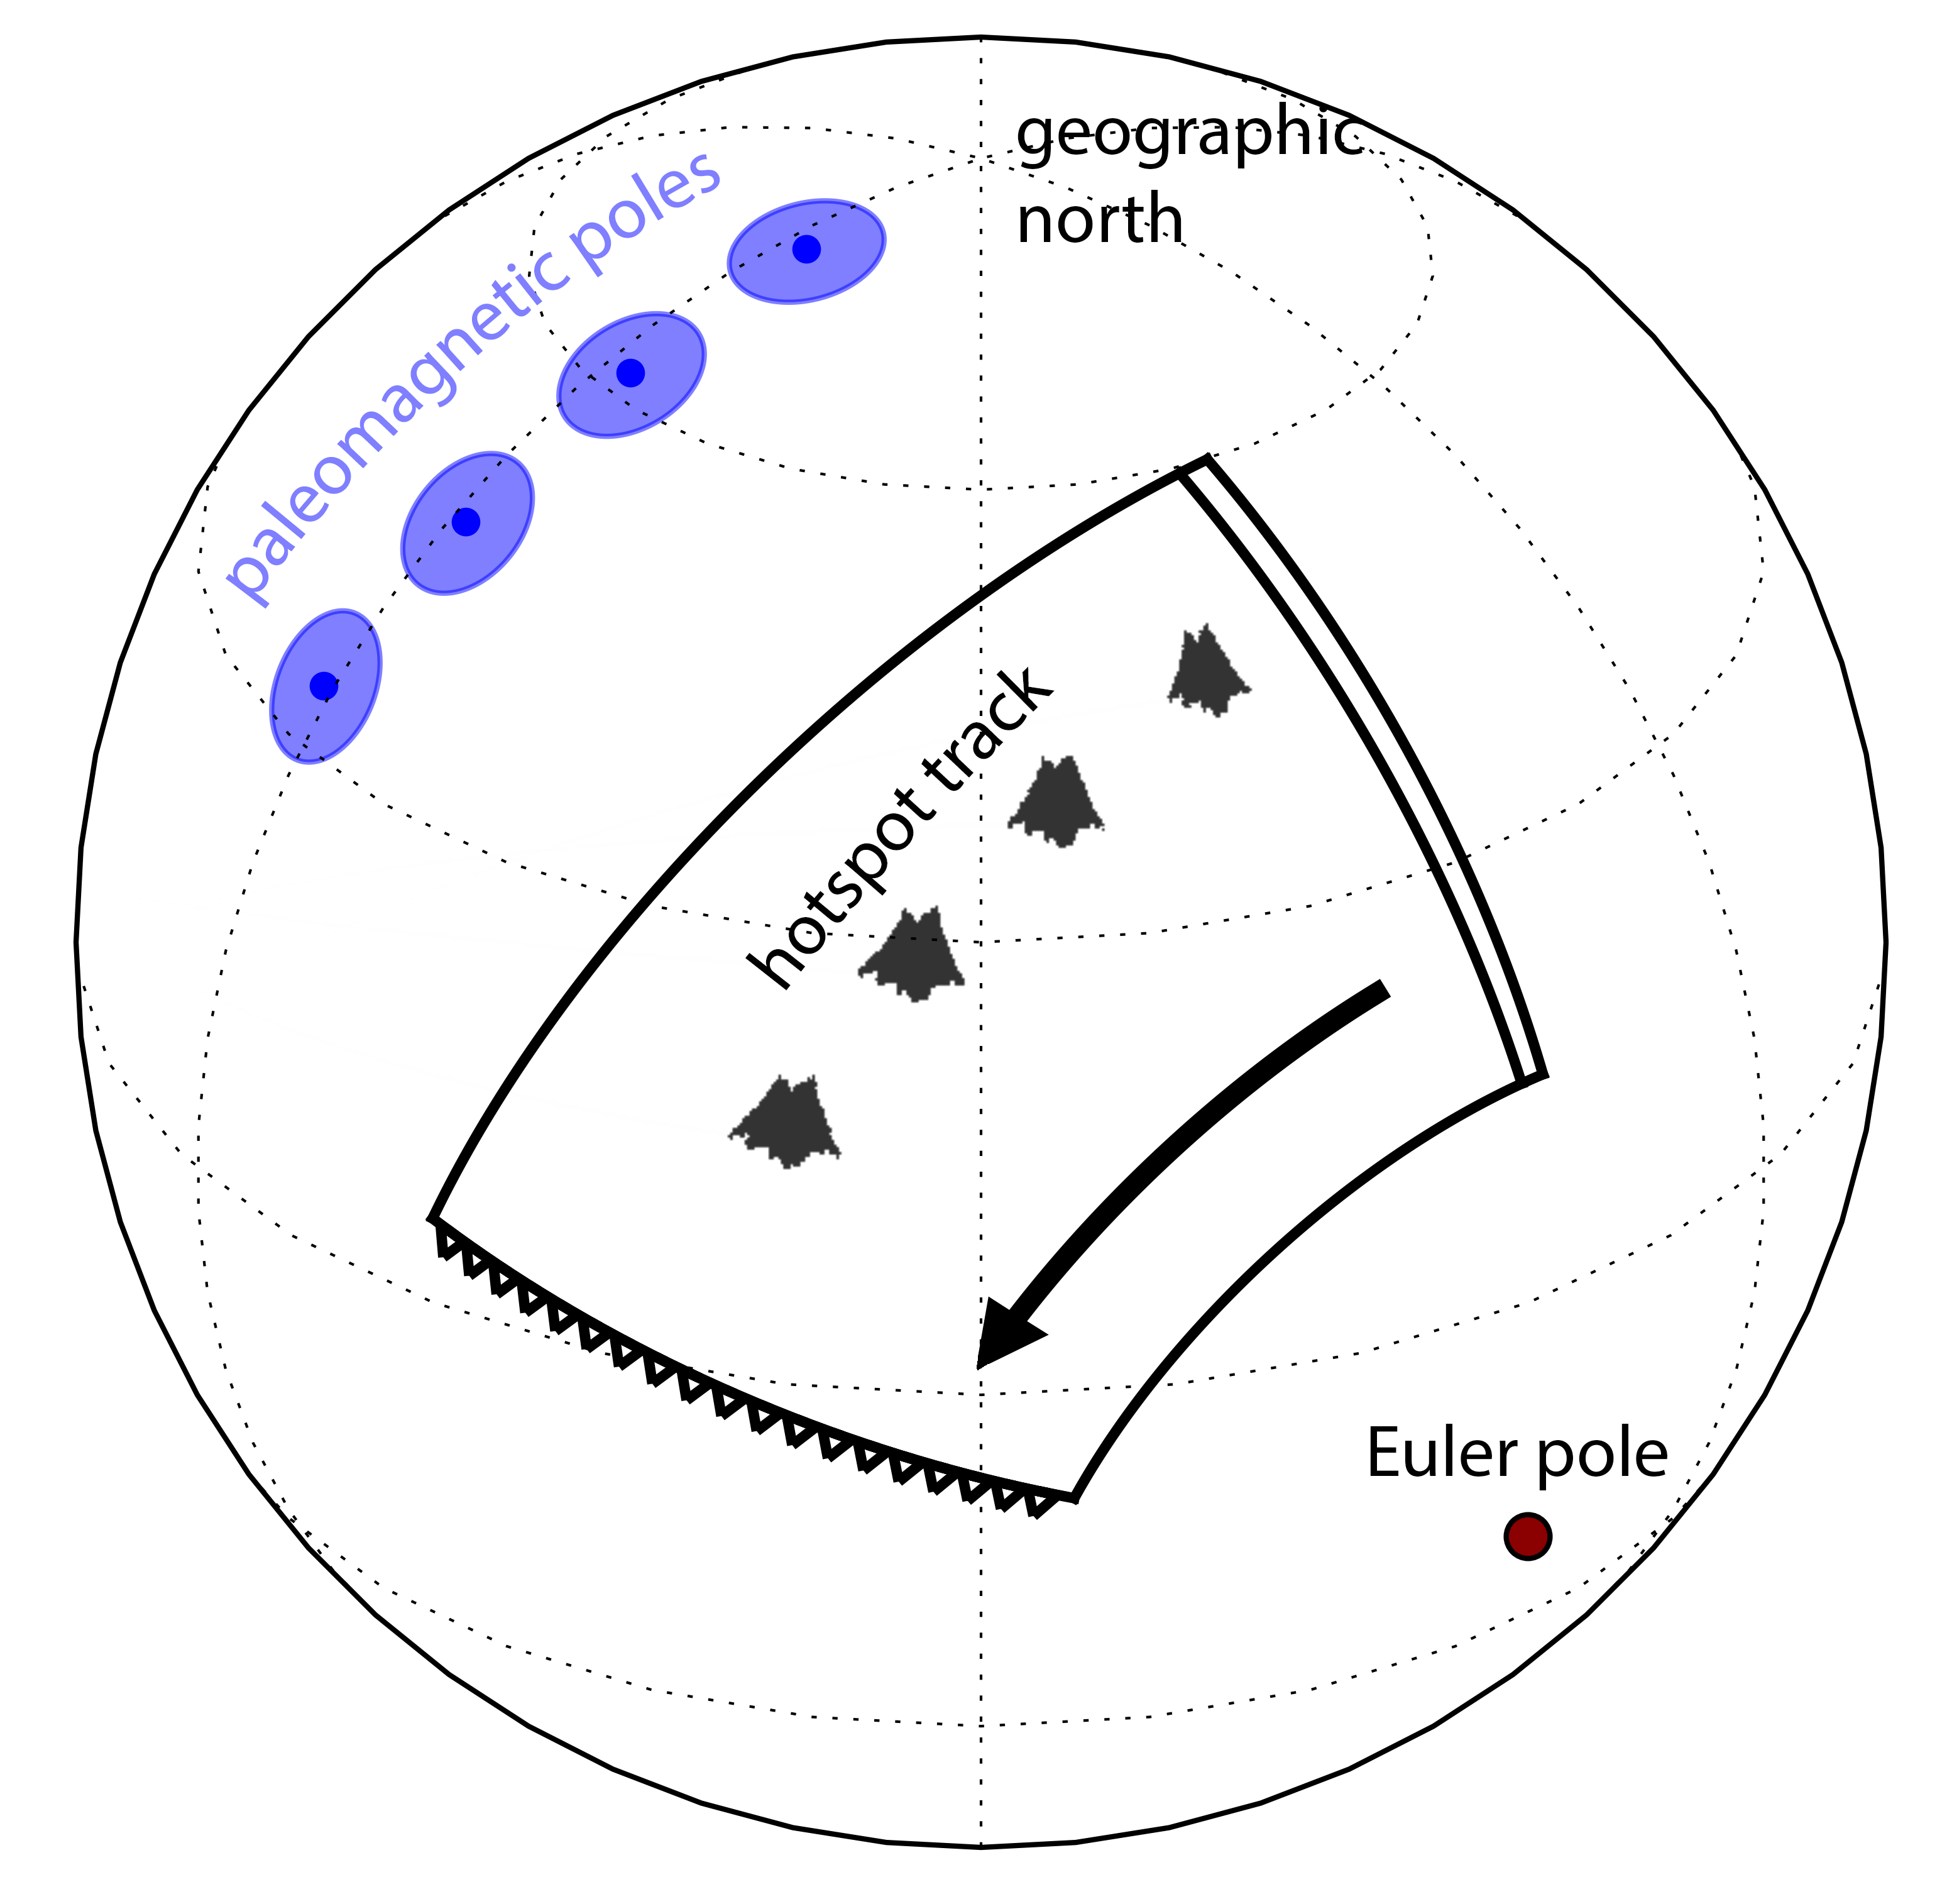
\includegraphics[width=0.5\textwidth]{fig_PEP_annotated.png}
\caption{Conceptual model for a paleomagnetic Euler pole. A finite rotation of a plate around an Euler pole (dark red circle) results in arcuate oceanic fracture zones and hotspot tracks (cartoon mountain) which describe small circles on the globe. The same finite rotation produces a circle in the APWP, which is illustrated by blue paleomagnetic poles. By fitting a small/great circle to the APWP, we may recover the Euler pole that produced the rotation which is termed the paleomagnetic Euler pole. Cartoon is adapted from \citeA{Gordon1984a}.}
\label{fig:pep}
\end{figure}

In this contribution, we extend paleomagnetic Euler pole analysis by placing it within a Bayesian statistical framework and demonstrate how to invert for paleomagnetic Euler poles using Markov chain Monte Carlo (MCMC) methods. This framework has the advantage of naturally incorporating uncertainties in paleomagnetic pole positions, as well as widely disparate age uncertainties associated with individual paleomagnetic poles. The resulting stage poles from these inversions are not a single answer, but are instead a distribution of possible answers, furnishing uncertainties as part of the solution process. Proper treatment of uncertainties also allow researchers to avoid overfitting models to noise. For instance, \citeA{Iaffaldano2012a} employed a similar Bayesian approach to inversions for finite plate rotations. They used seafloor data to reconstruct relative plate motion across Atlantic, Indian and South Pacific ridges incorporating uncertainties into the inversion. In the process, they demonstrated that interpretations of changes in relative plate motions on timescales $<$1 Myr are the result of overfitting the data and concluded there are fewer kinematic changes and longer stability in plate motions than suggested by some previous treatments.

In the sections below, we first review different approaches that have been applied to synthesize and interpret APWPs. We then describe the formalism of Bayesian inversions and Markov chain Monte Carlo methods that we will apply. We then describe the statistical model which we will be inverting and demonstrate the inversion of several synthetic data sets. Finally, we show case studies where we apply the method to paleomagnetic poles in order to develop estimates of paleomagnetic Euler poles and associated plate motion.

\section{Interpretation of apparent polar wander paths}

A sequence of paleomagnetic poles from the same continental block can be synthesized into an APWP, which can then be used to develop plate tectonic reconstructions and models of plate motion with respect to Earth's spin axis through time. Interpretation of these paths becomes difficult in the case of limited, uncertain, or conflicting data, and when the ages of paleomagnetic poles are poorly known. A number of approaches to developing APWPs have been developed, which we briefly review here.

\subsection{Latitudinal drift}
A paleomagnetic pole provides constraints on the paleolatitude and orientation of a lithospheric block. However, due to the rotational symmetry of Earth's time-averaged geocentric axial dipole magnetic field, paleomagnetic poles do not directly constrain absolute paleolongitude \cite{Butler1992a}. The simplest analysis of an APWP is to compare the paleolatitudes implied by successive poles for a point on a respective block. The difference in paleolatitudes gives a minimum angular distance over which the block has traveled. When this distance is compared to the age difference between the poles, such a comparison establishes a rate of latitudinal motion.

It is possible to estimate confidence bounds on the rate of latitudinal drift through bootstrap resampling \cite<e.g.>{Tarduno1990b} or by taking a Monte Carlo approach. \citeA{Swanson-Hysell2014b} developed a Monte Carlo sampling method and applied the method to a pair of poles from the Proterozoic Midcontinent Rift of North America to estimate the range of implied latitudinal drift. They also sampled from the uncertainties of radiometric dates associated with the poles, assuming Gaussian distributions, in order to incorporate age uncertainties into the analysis. With samples of pole position and ages, they were able to estimate the 95\% confidence estimates on the rate of latitudinal drift.

Whether using point estimates of the latitudinal drift rate or using Monte Carlo estimates, the latitudinal drift interpretation of APWPs remains limited as it represents a minimum estimate of total plate motion. It does not resolve longitudinal drift rate, nor does it naturally extend to APWPs with more than two poles, especially if two coeval poles are not in agreement, as it requires the selection of pole pairs.

\subsection{Spherical splines}
When considering APWPs with many poles, it becomes more difficult to perform latitudinal comparisons between pairs of poles. It is not always clear which pairs of poles to compare in cases where there are many overlapping paleomagnetic poles that have variable uncertainties associated with their positions and ages.

One approach to synthesize such data is to fit a spline through the set of paleomagnetic poles, constraining the path to lie on the surface of a sphere. This approach was pioneered by \citeA{Torsvik1992a} using the spherical spline algorithm developed by \citeA{Jupp1987a}. This approach has the advantage of allowing the paleomagnetic poles to be weighted by their spatial uncertainties. The uncertainty assigned to a paleomagnetic pole can be the 95\% confidence interval on the pole position, but it can also be augmented by various quality screening factors, such as the quality (``Q'') factor of \citeA{Van-der-Voo1990a} \cite{Torsvik1992a}. Even with the weighting of the paleomagnetic poles by uncertainty, there can be unrealistic loops in the APWP generated by the spline fit. To combat this behavior, the spline can also be computed under tension which penalizes curvature and produces a smoother path \cite{Torsvik1996a}.

The spherical spline approach to interpreting APWPs has attractive features. It produces a smooth path through the data that can incorporate spatial uncertainties, and may be efficiently computed. However, it does have some drawbacks. It is not easy to determine the appropriate uncertainty weighting and spline tension parameters for the fit, and what effect those choices have on the result. Furthermore, the resulting fit does not have an uncertainty with a physically interpretable meaning \cite{Torsvik1996a}. It also does not have a simple way of incorporating age uncertainties of the paleomagnetic poles. Finally, by their nature, splines do not readily represent the sharp hairpin cusps that characterize abrupt shifts in motion that plates sometimes undergo \cite{Irving1972a, Gordon1984a, Torsvik2012a}.

\subsection{Running means}

An alternative method for developing APWPs is to perform a running Fisher mean on the poles with a moving window through time \cite{Irving1977a, Van-der-Voo2001a, Torsvik2008a}. In such an analysis, paleomagnetic poles in a compilation are averaged with a defined window duration (typically 10-30 Myr) that controls the amount of smoothing. Like spherical splines, the running mean approach has the ability to effectively damp the effect of outlier poles that could lead to spurious motion in the APWP if there are sufficient data. \citeA{Torsvik2008a} also investigated the effects of combining running means with spherical splines, by first computing a set of mean poles and then fitting a spline through those means. The simplicity of using the running mean approach to develop an APWP, as well as its ability to suppress potentially spurious poles, has led to it being widely adopted.

While it is a straightforward approach with advantages for synthesizing paleomagnetic poles, the running mean approach shares many of the drawbacks of the spline approach. As with the spherical spline method, age uncertainties on the poles are not incorporated, nor are the uncertainties in pole positions as typically implemented. It is not obvious how to best choose the window duration, and different window durations are likely appropriate for different data sets. It is also unclear how to interpret the resulting uncertainties in the path that are reported as a Fisher A$_{95}$ ellipse of the mean of the poles as the poles need not be coming from a Fisher distribution particularly if there is ongoing plate motion. A recent study discussed the advantage that could be gained by calculating APWPs from site level data (virtual geomagnetic poles) rather than from study level mean paleomagnetic poles \cite{Vaes2022a}. This work highlighted how such an approach could ameliorate the disadvantage of typical running mean approaches of giving equal weight to study level poles which themselves comprise varying numbers of site level virtual geomagnetic poles.

\subsection{Paleomagnetic Euler poles}
The idea of fitting small circles to paleomagnetic data to gain insight into plate motions was first described by \citeA{Francheteau1969a}. The center of such a circle on a sphere is the pole of rotation which was termed a paleomagnetic Euler pole by \citeA{Gordon1984a} who developed a method to invert for the position of such poles. The approach builds on the recognition that plate motions can often be approximated by finite rotations around Euler poles which can potentially be steady for millions or tens of millions of years. As a result, an arcuate APWP of a plate can be described by Euler rotations, which produce small circle paths on Earth's surface if the Euler pole remains in a relative constant position (Fig. \ref{fig:pep}). Since the analysis solves for the Euler pole that produces a given small circle, this approach allows for an estimate of the full motion of a given plate, including the total plate speed (instead of just the latitudinal component of the speed). Effectively, the analysis utilizes both the change in plate orientation and latitude information embedded within paleomagnetic poles to estimate both latitudinal and longitudinal motion as succinctly specified by Euler pole parameters.

However, paleomagnetic Euler pole analysis has many of the same deficiencies that spline fits and running means have---it is not easy to compute uncertainties, especially in the presence of unknown ages of poles. Furthermore, one has the additional challenge and related uncertainty of deciding how many paleomagnetic Euler poles to include for a given sequence of paleomagnetic poles. In most treatments, this number of stage poles is subject to researcher choice (however, see theoretical progress in this regard by \citeA{Gallo2022a}). In this contribution, we develop a Bayesian statistical approach to paleomagnetic Euler pole analysis which attempts to address some of these deficiencies.

\section{Bayesian inversion}
\subsection{A general description of inverse problems}

The central question motivating inverse problems is ``How probable is a particular model, given my observations?''. We represent observations by the data vector $\mathbf{d}$, and a model by the vector of model parameters $\mathbf{m}$, so the above question can be expressed as the function $P(\mathbf{m} \vert \mathbf{d})$ (the probability of the model given the data). Traditional frequentist approaches to an inverse problem often proceed by maximizing the likelihood function, defined by the probability of the data given a particular model \cite<e.g.>{Aster2005a}:
\begin{equation}
\mathcal{L} ( \mathbf{m} \vert \mathbf{d} ) \equiv P( \mathbf{d} \vert \mathbf{m} ).
\label{eq:likelihood}
\end{equation}
The likelihood function replaces something that is difficult to compute (namely, $P(\mathbf{m} \vert \mathbf{d})$)
with something that is less difficult to compute. 
To compute $\mathcal{L}(\mathbf{m} \vert \mathbf{d})$ we need to have two things: a statistical model for 
uncertainties in the observations $\mathbf{d}$ and a forward model that allows us to compute
predictions. We denote the forward model by $\mathbf{g}$:
\begin{equation}
\mathbf{d}^p = \mathbf{g}(\mathbf{m}),
\label{eq:forward}
\end{equation}
where the superscript ``$p$'' denotes a predicted value.
If each of the observed data $d_i$ are described by Gaussian random variables with standard deviations $\sigma_i$, the likelihood function is given by the product of the individual likelihoods of the observations:
\begin{equation}
\mathcal{L}(\mathbf{d} | \mathbf{m} ) = \displaystyle\prod_i \exp\left({-\frac{(d_i - d_{i}^p)^2}{2 \sigma_i^2}}\right).
\label{eq:example_likelihood}
\end{equation}
The likelihood function $\mathcal{L}$ is maximized by searching over the model parameter space.
If the uncertainties in the observations are Gaussian, then maximizing the likelihood function is
equivalent to the least squares solution \cite{Aster2005a}.

A standard maximum likelihood fit will frequently overfit the observations, resulting in unrealistic solutions. In the context of APWPs, these overfit solutions may pass through every paleomagnetic pole, including less reliable ones, resulting in loopy or jerky paths. In order to address such overfitting, some form of regularization is usually included in the solution of the inverse problem, such as penalizing the magnitude or curvature of the solution. Both the running-mean and the spline under tension approaches to APWPs are forms of regularization on the problem.

\subsection{Bayesian approach}

The Bayesian approach to inverse problems takes a different strategy from the frequentist one. Rather than finding a model with parameters that maximize the likelihood, it treats the underlying model as a set of random variables with individual probability distributions. The probability distribution of the model given the data ($P(\mathbf{m} \vert \mathbf{d})$) is then found by an application of Bayes theorem \cite<cf.>{Sivia2006a}:
\begin{equation}
P\left(\mathbf{m} \vert \mathbf{d} \right) = \frac{ P \left(\mathbf{d}\vert \mathbf{m} \right) P \left( \mathbf{m} \right) }{P \left( \mathbf{d}\right).}
\label{eq:bayes}
\end{equation}
It is often unnecessary to calculate the denominator of Equation~\ref{eq:bayes}, which is a normalization constant, leaving us with
\begin{equation}
P\left(\mathbf{m} \vert \mathbf{d} \right) \propto P \left( \mathbf{d} \vert \mathbf{m} \right) P \left( \mathbf{m} \right).
\label{eq:propbayes}
\end{equation}
The quantity $P(\mathbf{m} \vert \mathbf{d})$ is known as the posterior probability, and it represents our desired knowledge about the distributions of the parameters $\mathbf{m}$. The first factor on the right-hand-side of Equation~\ref{eq:propbayes} is identical to the likelihood function described above, and the second factor
is known as the prior probability of the model. In the case for Euler pole and/or true polar wander inversions, our model parameters are Euler pole positions (longitudes, latitudes) and rotation rate as well as changepoints (when multiple rotations are inverted for). 

%Therefore, $P(\mathbf{m} \vert \mathbf{d})$  can be rewritten as $P\left(\mathbf{Euler\ poles, Euler\ rates, changepoints, pole\ ages} \vert \mathbf{paleomagnetic\ poles} \right)$, $P(\mathbf{d} \vert \mathbf{m})$ can be rewritten as $P \left( \mathbf{paleomagnetic\ poles} \vert \mathbf{Euler\ poles, Euler\ rates, changepoints, pole\ ages} \right)$, and $P(\mathbf{m})$ can be rewritten as $P \left( \mathbf{Euler\ poles, Euler\ rates, changepoints, pole\ ages} \right)$.
% \begin{equation}
% P\left(\mathbf{Euler\ poles, Euler\ rates, changepoints} \vert \mathbf{paleomagnetic\ poles, pole\ ages} \right) \\ \propto \\ P \left( \mathbf{paleomagnetic\ poles, pole\ ages} \vert \mathbf{Euler\ poles, Euler\ rates, changepoints} \right) P \left( \mathbf{Euler\ poles, Euler\ rates, changepoints} \right).
% \label{eq:propbayes}
% \end{equation}

In this case, the prior probability distributions reflect the state of our knowledge and beliefs of the values of the Euler rotation axes and rotation rates prior to the consideration of data. It allows us to incorporate theoretically or empirically derived constraints that are not otherwise included in the forward model. In contrast with the classical statistical approach of regularization, the Bayesian inverse problem can (in effect) regularize the problem by making
choices of probability distributions that have less probability density in parameter space with less realistic values \cite<e.g.>{Minson2013a, Sambridge2013a}.

\subsection{Markov chain Monte Carlo methods}

For complex models, it is usually impossible to calculate the posterior probability distribution in Equation~\ref{eq:bayes} directly \cite{Davidson-Pilon2015a}. It is much more tractable to generate a Markov chain which, upon convergence, generates samples from the desired posterior distribution \cite{Gelman2013a}. This approach defines a class of methods known as Markov chain Monte Carlo (MCMC) methods. 

In comparison with drawing Monte Carlo resamples from random variables independently, Markov chain Monte Carlo resampling generates a sequence of samples where the current value for each variable is dependent on its prior value. This approach allows for more efficient sampling of probability distributions with sampling that converges towards higher posterior probabilities. For an introduction to MCMC methods, the interested reader could refer to \citeA{Gelman1996a}, \citeA{Sambridge2013a}, and \citeA{Davidson-Pilon2015a}. A number of high-quality open source software packages for implementing MCMC models exist, including WinBUGS \cite{Lunn2000a}, PyMC \cite{Salvatier2016a}, and Stan \cite{Carpenter2017a}. We make extensive use of PyMC in this work.

\subsection{Distributions on a sphere}

In order to proceed with a Bayesian description of the problem, every parameter in the model needs to be described by some statistical distribution that determines the probability that the parameter takes a specific value. Parameters like pole ages can be described by 1D probability distributions (such as uniform or normal distributions), whereas Euler pole locations are described by 2D distributions of directional data on the surface of a sphere. We review several of these distributions here. For a comprehensive discussion of spherical probability distributions, see \citeA{Fisher1987b}. Plots of the following distributions (uniform, Fisher, and Watson), as well as samples drawn from them, are shown in Figure \ref{fig:distributions}. 

\subsubsection*{Uniform distribution}
\begin{figure*}
\centering
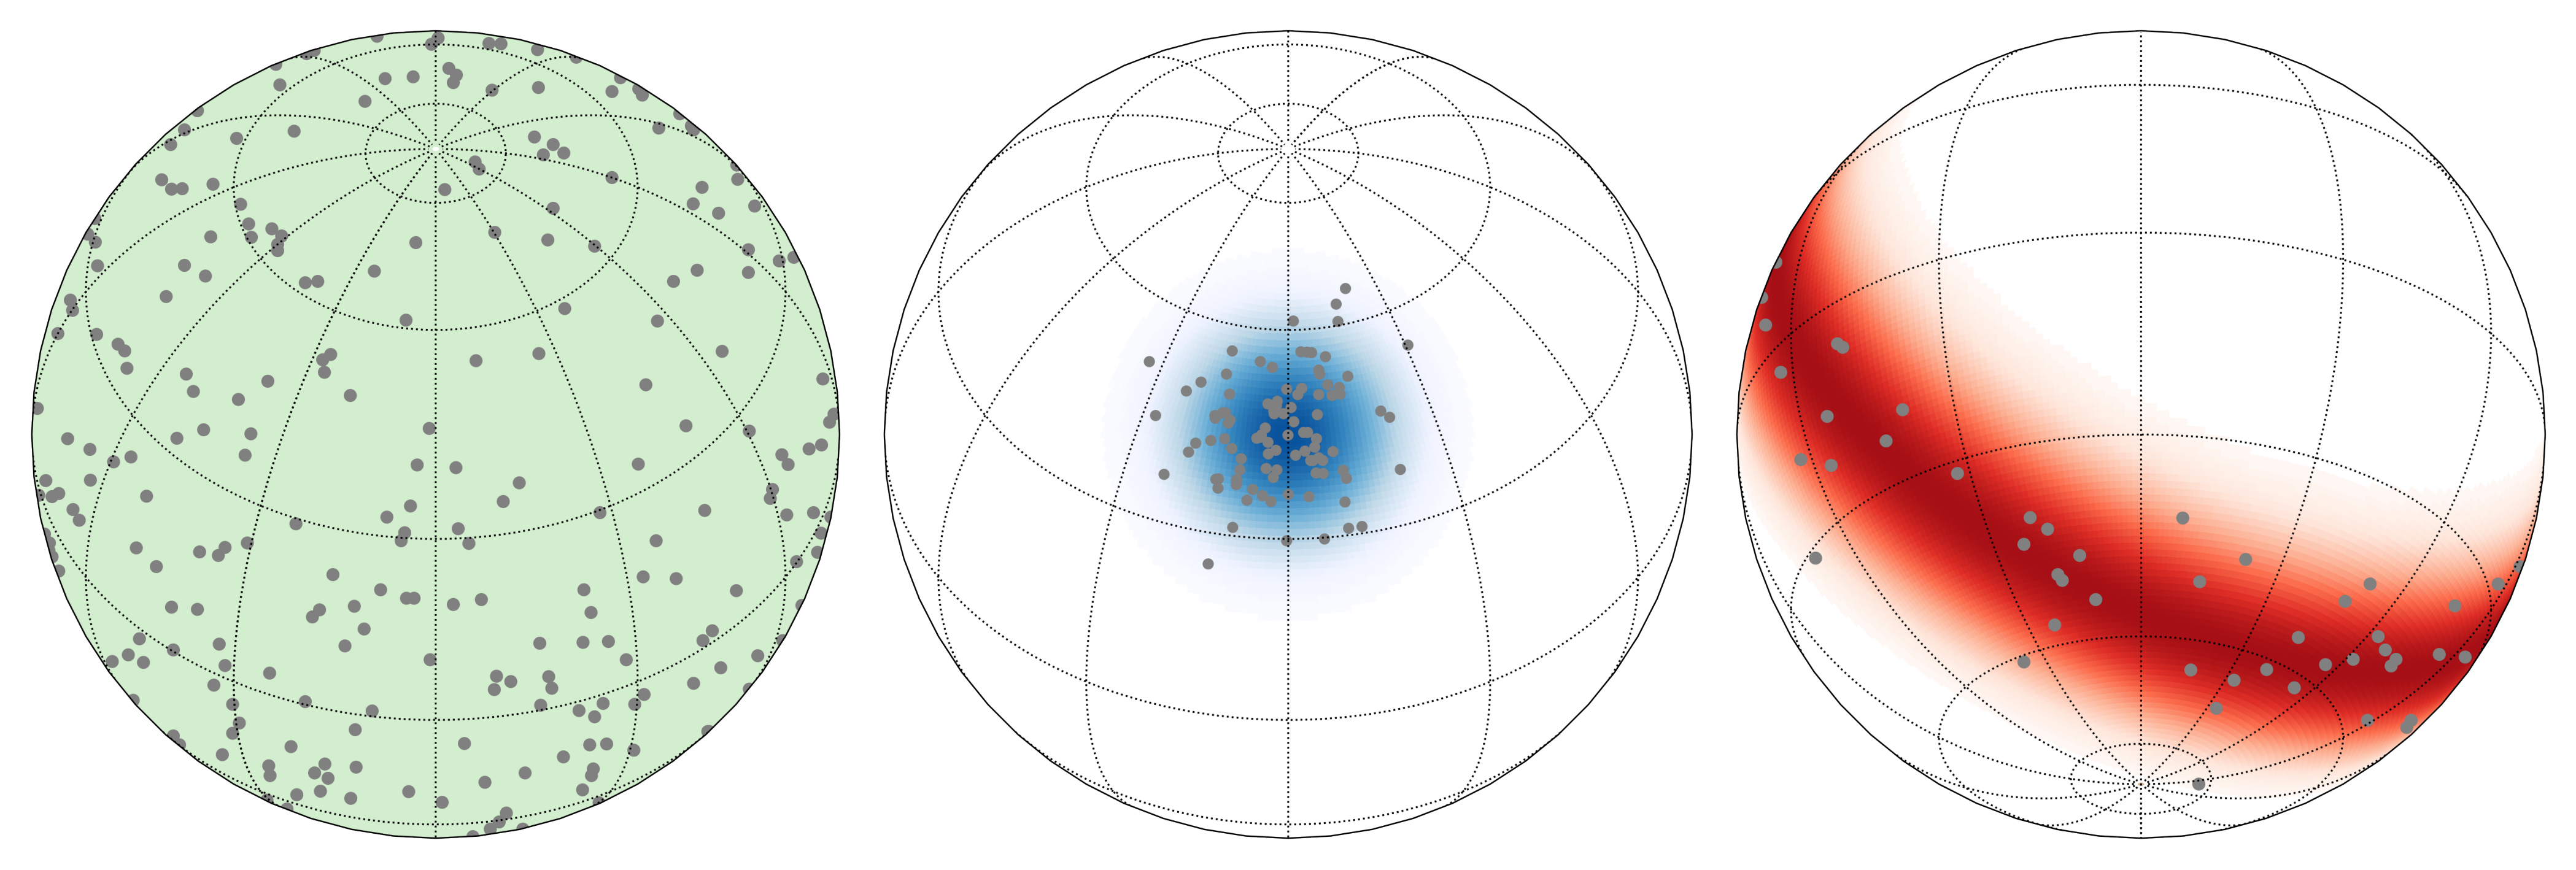
\includegraphics[width=\textwidth]{fig_direction_distributions.png}
\caption[Spherical probability distributions.]{Probability densities for distributions of directional data, as well as samples drawn from them. All distributions are plotted using an orthographic projection. (left panel) Uniform distribution. (middle panel) Fisher distribution. The center of the distribution is at $45^\circ$N, $30^\circ$E, with concentration parameter of $\kappa_F=50$. (right panel) Watson girdle distribution. The pole of symmetry is at $30^\circ$N, $30^\circ$E, with a concentration parameter of $\kappa_W=-25$.}
\label{fig:distributions}
\end{figure*}

The simplest probability distribution on a sphere is the spherical uniform distribution. It has a probability density given by
\begin{equation}
  \rho_U(\phi, \psi) = \frac{1}{4 \pi} \cos \psi 
\ or \
  \rho_U(\hat{\mathbf{x}}) = \frac{1}{4 \pi}
\end{equation}
where $\rho_U$ is the probability density, $\phi$ is the longitude, and $\psi$ is the latitude (we refer to the Cartesian unit vector $\hat{\mathbf{x}}$ as a concise representation of $\phi$ and $\psi$). Non-uniform distributions on a sphere reduce to the uniform distribution in some limit (i.e. the Fisher distribution as the precision parameter goes to zero). We use the uniform distribution when we want to specify an uninformative prior distribution for directional parameters.

\subsubsection*{Fisher distribution}
The Fisher distribution (also called the von Mises-Fisher distribution) is the analogue of a 2D normal distribution on a sphere (Fig. \ref{fig:distributions}). The probability density $\rho_F$ at a point $\hat{\mathbf{x}}$ is given by
\begin{equation}
  \begin{aligned}
  \rho_F(\phi, \psi ; \kappa_F, \hat{\mathbf{\mu}}) 
  &= \frac{1}{C_F} \exp \left( \kappa_F \hat{\mathbf{x}}^T \hat{\mathbf{\mu}} \right) \\
  &= \frac{1}{C_F} \exp \left( \kappa_F \cos \theta \right),
  \end{aligned}
\end{equation}
where $\kappa_F$ is the concentration of the distribution, 
$\hat{\mathbf{\mu}}$ the unit vector for the mean direction of the distribution, and $C_F$ is a normalization coefficient. It can be alternatively parameterized using $\theta$, which is the angle between $\hat{\mathbf{x}}$ and $\hat{\mathbf{\mu}}$.
The normalization factor is given by 
\begin{equation}
  C_F = \frac{\kappa_F}{4 \pi \sinh{\kappa_F}}.
\end{equation}
When $\kappa_F$ goes to zero, the Fisher distribution is equivalent to the spherical uniform distribution.

The uncertainty ellipses for paleomagnetic poles are typically calculated assuming a Fisher distribution of the underlying data, and we will use this distribution to calculate the likelihood function for pole positions in the model.

\subsubsection*{Watson girdle distribution}
Whereas the Fisher distribution concentrates probability density around a pole on the surface of the sphere, the Watson girdle probability distribution is concentrated in a belt orthogonal to the pole (Fig. \ref{fig:distributions}). It is useful for characterizing planar data, and is given by
\begin{equation}
  \begin{aligned}
  \rho_W(\phi, \psi; \kappa_W, \hat{\mathbf{\mu}}) 
  &= \frac{1}{C_W} \exp \left( \kappa_W (\hat{\mathbf{x}}^T \hat{\mathbf{\mu}})^2 \right) \\
  &= \frac{1}{C_W} \exp \left( \kappa_W \cos^2 \theta \right),
  \end{aligned}
\label{eq:watson}
\end{equation}
where $\kappa_W$ is the concentration of the girdle, $C_W$ is a normalization coefficient, and the other parameters are identical to those in the Fisher distribution. The Watson distribution is girdle-shaped only when $\kappa_W$ is a negative number, which is the only case we consider here.

The normalization factor is given by
\begin{equation}
  C_W = \left[ {}_1 F_1 \left( \frac{1}{2}, \frac{3}{2}, \kappa_W \right) \right]^{-1},
\end{equation}
where ${}_1 F_1()$ is Kummer's confluent hypergeometric function, which is available in most software libraries of special mathematical functions. As with the Fisher distribution, when $\kappa_W$ goes to zero,  the Watson distribution is equivalent to the spherical uniform distribution.

\section{A model for paleomagnetic Euler pole inversion}
\label{sec:model}
\subsection{Forward model}
\label{sec:forward_model}
A forward model describes how we generate predicted observations given a set of model parameters (Equation~\ref{eq:forward}). The forward model for paleomagnetic Euler pole analysis in this study is essentially unchanged from that of \citeA{Gordon1984a}. We will consider three overall scenarios of plate motions (and hence paleomagnetic pole motions). The first is that plate motion is the result of plate tectonic motion about an Euler pole or a series of Euler poles. Each Euler pole has three parameters: a latitude, a longitude, and a rotation rate. In a model with multiple Euler poles, we also must specify the ages where one Euler pole switches to the next as an additional unknown variable. In the context of parameter inversion, these ages are often known as ``changepoints.'' For plate tectonic motions, the motion can be along any plane intersecting the sphere such that they are small circles. The second scenario we will consider is one wherein the sole cause of the motion of paleomagnetic poles is true polar wander in which case motion is restricted to be along a great circle path coaxial to the axis of minimum inertia \cite{Creveling2012a}. In such a model, three parameters exist: a latitude and a longitude of the true polar wander rotation axis and a rotation rate.  A third scenario is that plate tectonic and true polar wander rotations are occurring concurrently leading to an observed paleomagnetic pole path. 

We also need to initiate a model with a starting position on the globe, which, in practice, can be sampled from the Fisher distribution of the oldest paleomagnetic pole in the data set. The starting point contributes two parameters (a latitude and a longitude). 

Therefore, a model with $n_e$ Euler rotations will have $3 n_e$ parameters for the poles, $(n_e-1)$ parameters for the changepoints, and 2 parameters for the starting location. The number parameters for which we are inverting is then given by
\begin{equation}
\begin{aligned}
N &= 3 n_e + (n_e -1) + 2 \\
 &= 4 n_e + 1.
\end{aligned}
\label{eq:n_parameters}
\end{equation}

Two more parameters will be included in a model where true polar wander is considered to happen on top of $n_e$ Euler rotations. In this case, the axis of true polar wander is constrained to be on a great circle that is orthogonal to the vector representing the starting pole position. Therefore, a total of $4 n_e + 3$ parameters are inverted for. 

With the axes and rates for such spherical rotations defined, one can calculate the linear velocity $\mathbf{v}$ of a point $\mathbf{p}$ on the surface of the globe associated with angular velocity $\mathbf{\omega}_i$ by
\begin{equation}
\mathbf{v} = \mathbf{\omega}_i \times \mathbf{p}.
\label{eq:rigid_rotation}
\end{equation}

%On top of these parameters associated with spherical rotations, we can also incorporate ages associated with each observed paleomagnetic pole in the forward model. In a case where a portions of the paleomagnetic poles have good age constraints (such as a radiometric date derived from the parent rock) whereas the rest of the poles have poorly constrained ages, the posterior distributions given by the Bayesian inversion model could provide an estimate on the ages of all poles in a particular model setup.

Finite rotations can be performed by constructing Euler angle rotation matrices \cite<cf.>{Goldstein1965a}.  We generate synthetic paleomagnetic pole positions from the forward model by stringing together finite rotations through the stage poles until the age of the observed paleomagnetic pole is reached. These positions can then be compared to the observed paleomagnetic poles in a given dataset.

\subsection{Choice of prior distributions}
\label{sec:priors}

Bayesian analysis requires us to specify prior probability distributions for each of the model parameters in the inverse problem. These distributions reflect our state of knowledge about the values of the parameters before we begin, and allow us the option of incorporating information otherwise not captured by the model. To avoid biasing the results of the model towards a specific posterior distribution, we usually try to choose prior distributions that are as uninformative as possible. Depending upon the context, and the type of parameter, that choice may vary. The central parameters in the paleomagnetic Euler pole problem are the Euler pole positions, the Euler pole magnitudes, the changepoints, the starting point, and the paleomagnetic pole ages, which we treat in turn. We use the notation $x \sim y$ to indicate that the parameter $x$ is drawn from distribution $y$.

\textbf{Euler rotation vectors:} 
The first parameter we consider is the position of the Euler poles, which should be drawn from a spherical probability distribution. The least informative prior distribution for an Euler pole position is the uniform spherical distribution:
\begin{equation}
\hat{\mathbf{\omega}}_i \sim \rho_U.
\end{equation}
essentially allowing the Euler pole to be anywhere on the globe with equal probability.

An alternative choice is to inform our prior distribution for Euler pole positions based on observation of modern plate motions. It has long been observed that, to first order, plate motions are well explained by slab-pull torques acting along subduction zones, and to a lesser extent, ridge push and mantle traction effects \cite{Forsyth1975a, Gordon1978a, Richardson1992a}. 

We can ask the question of whether the Euler pole for a given plate is more likely to be on top of the plate (corresponding to a spinning motion for that plate) or away from that plate (corresponding to motion across the surface of Earth). Given that tectonic plates can broadly be considered to be the surface expression of mantle convection, we can hypothesize that the second possibility is more likely because a spinning plate has no divergence (i.e., spreading centers and subduction zones, \cite{Forte1987a, Gable1991a}. Without divergence, the plate motion does not contribute to large-scale convection.

To evaluate this hypothesis, we generated position samples on the surface of Earth and computed the angular distance between that point and the Euler pole for the plate in which that point resides. We used the NNR-MORVEL56 model for current plate motions \cite{Argus2011a} and restricted our analysis to the fourteen largest plates. We then fit those angular distance samples to a Watson girdle distribution (Equation~\ref{eq:watson}),  inverting for the concentration parameter $\kappa_W$. If an Euler pole position has no preference for being a particular angular distance from a point on a plate, then $\kappa_W$ should be close to zero, corresponding to a uniform distribution. We find that the distribution is best fit with $\kappa_W \approx -0.7$, which corresponds to the Euler pole probability density being roughly twice as large $90^\circ$ away from a given point than on top of the point (Fig.~\ref{fig:euler_pole_prior}).

\textbf{Euler rotation magnitudes:} 
The magnitude of each Euler pole rotation is a positive number, specifying the rotation rate about the Euler pole (negative magnitudes can be accommodated by flipping an Euler pole to the antipode). There are several possibilities for the prior distribution for the rates. In order to not bias the inversion towards a particular rate, we can choose a uniform prior distribution with large support:
\begin{equation}
\vert \mathbf{\omega}_i \vert \sim U(\cdot, \cdot),
\end{equation}
where $U(\cdot, \cdot)$ is a uniform distribution between two values, and is specified in degrees per million years. Typical rotation rates for present day plate motions are under $1^\circ$/Myr \cite{Argus2011a}, which corresponds to plate speeds of about 11 cm/yr for a rotation about an Euler pole that is $90^\circ$ from a plate.

Another option is to choose a weakly informative prior distribution for the Euler pole magnitudes informed by recent plate motions (similar our approach of the Watson girdle prior distribution for Euler pole position). \citeA{Zahirovic2015a} found, based on analysis of Cenozoic and Mesozoic plate reconstructions, that plate speeds much higher than 15 cm/yr were unlikely to be sustained. A reasonable choice of distribution for strictly positive numbers is the exponential distribution, given by
\begin{equation}
\rho_E(\vert \mathbf{\omega}_i \vert) = \lambda \exp(-\lambda \vert \mathbf{\omega}_i \vert),
\end{equation}
which has higher probability density at lower values, and falls off exponentially toward higher values. We sampled the current plate rates on Earth's surface according to NNR-MORVEL56 and fit those to an exponential distribution. The best fitting scale parameter $\lambda$ for current plate rates is $\sim2.5$ (Fig.~\ref{fig:euler_pole_prior}). Making this choice of prior distribution for Euler pole rotation rates can be seen as a form of regularization on plate speeds. A smaller for $\lambda$ (such as $\lambda =1$ as is shown in Fig.~\ref{fig:euler_pole_prior}) could reflect similar knowledge about the distribution of plate speeds with a less restrictive regularization.

\begin{figure*}
\centering
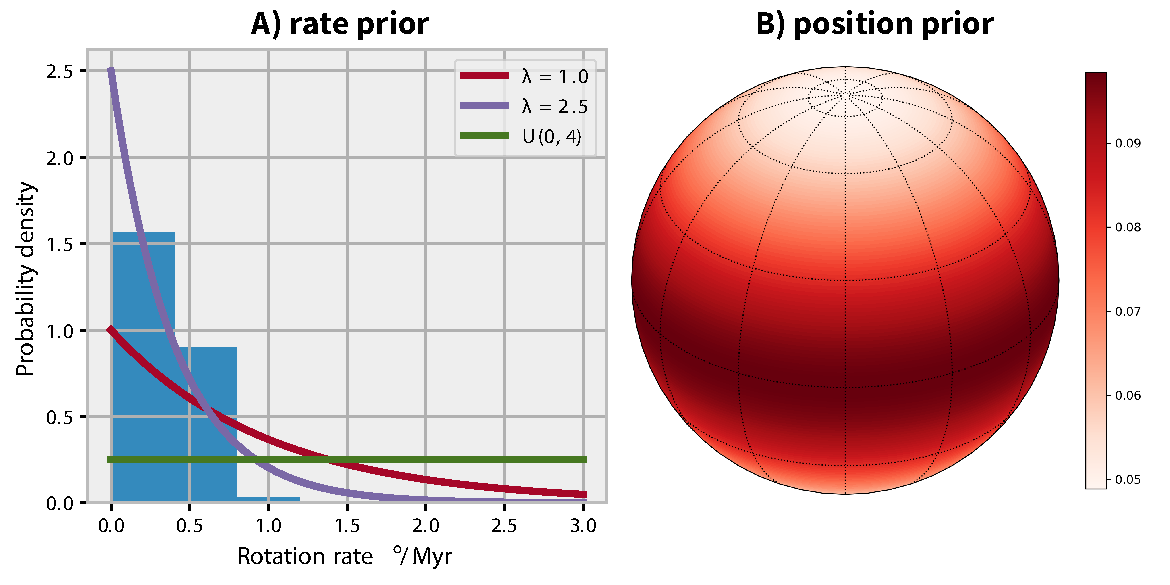
\includegraphics[width=0.9\textwidth]{fig_euler_pole_prior.pdf}
\caption[Informative prior distributions for Euler poles]{Informative prior distributions for Euler poles. (a) Prior probabilities for rotation rates. The histogram is the angular rotation rate from one thousand samples from the surface of Earth, using the NNR-MORVEL56 model. A fit to this sample set with an exponential distribution yields a scale parameter of $\lambda \approx 2.5$. We also show the distribution for $\lambda = 1.0$, which imposes less regularization on the rate as a less restrictive prior distribution, and a uniform $U(0,4)$ distribution between 0 and 4\textdegree/Myr, which specifies no preference for slower speeds if set as the prior probability. (b) Prior probability density for the position of the Euler poles, with the north pole as the site latitude and longitude.  We again sampled one thousand points on Earth's surface, calculating the angular distance between that point and the Euler pole for its plate.  If we model the probability distribution as being drawn from a Watson distribution, these angular distances correspond to colatitudes, where the pole is the sampled point.  Fitting the resulting angular distribution to a Watson girdle distribution finds $\kappa_W\approx-0.7$. Since the Watson distribution is rotationally symmetric, longitudes do not contribute to the fit. For $\kappa_W\approx-0.7$ the probability density is roughly twice as large at the equator (90\textdegree\ from a plate) as at the pole (on top of the plate).}
\label{fig:euler_pole_prior}
\end{figure*}

\textbf{Changepoints:} 
Changepoints occur sequentially between the oldest (at age $a_\mathrm{max}$) and youngest (at age $a_\mathrm{min}$) paleomagnetic poles. We choose a uniform distribution as a prior for these changepoints:
\begin{equation}
c_i \sim U( a_\mathrm{min}, a_\mathrm{max}),
\end{equation}
where $c_i$ is the i'th changepoint.

\textbf{Starting position:}
Finally, the starting position $\hat{\mathbf{x}}_\mathrm{start}$ for the set of Euler pole rotations needs a prior distribution. We could choose another uniform distribution, but a more reasonable choice is to start near the oldest paleomagnetic pole in the dataset. We therefore choose the Fisher distribution of the oldest paleomagnetic pole as a reasonable prior distribution for a start point:
\begin{equation}
\hat{\mathbf{x}}_\mathrm{start} \sim \rho_F(\kappa_{F0}, \hat{\mathbf{\mu_0}}),
\end{equation}
where $\kappa_{F0}$ and $\hat{\mathbf{\mu}}_0$ are the concentration parameter and mean direction of the oldest paleomagnetic pole in the dataset.

\textbf{Pole ages:}
One of the major advantages of Bayesian analysis is the ability to naturally incorporate uncertainties in as many parameters as needed. Previous approaches to modeling APWPs have the drawback that they do not easily account for uncertainties in the age of paleomagnetic poles. In our approach, we can include age uncertainty by including the age of the poles and associated uncertainty as parameters in our model.

There are many different ways to constrain the ages of the geologic units from which we obtain paleomagnetic poles, including radiometric dating, biostratigraphy, magnetostratigraphy, and cross-cutting relationships. Here we concentrate on poles that are either interpreted to be the age of a single radiometric date or are interpreted to be bracketed stratigraphically between two dates (derived radiometrically or by using other age control such as biostratigraphy). If a geologic unit has been radiometrically dated, we can model the age of the j'th paleomagnetic pole $a_j$ as a normal distribution with mean $\mu_j$ and standard deviation $\sigma_j$:
\begin{equation}
a_j \sim N(\mu_j, \sigma_j),
\end{equation}
where $N(.,.)$ denotes a normal distribution.

Frequently, however, the geologic unit from which we obtain a paleomagnetic pole is not well dated, but its age can be constrained to lie between those of well-dated units stratigraphically above and below it, dates obtained by cross-cutting relationships, or a number of dated units within a broader province. In these cases, a uniform distribution between those ages is a reasonable choice for the prior distribution:
\begin{equation}
a_j \sim U(a_\mathrm{young}, a_\mathrm{old}),
\end{equation}
where $a_\mathrm{young}$ and $a_\mathrm{old}$ are the ages of the lower and upper age constraints, respectively.

\textbf{True polar wander:}
Another advantage of this method is the ability to also incorporate a component of true polar wander rotation on top of Euler pole rotations. Because true polar wander represents the rotation of the entire solid Earth with respect to the spin axis, an APWP that is solely consisted of true polar wander should follow a great circle trajectory and the associated rotation axis should be orthogonal to the great circle. In a case where both small circle rotations and true polar wander are recorded by an APWP, the true polar wander rotation axis is constrained to be 90\textdegree\ away from the start position of the path and the rotation rate can be defined in a similar fashion as that of the Euler pole magnitudes.


To summarize our choices for prior distributions:
\begin{itemize}
\item Euler pole positions: spherical uniform distribution, or a Watson girdle distribution with $\kappa_W \approx -0.7$.
\item Euler pole magnitudes: Uniform distribution, or an exponential distribution with $\lambda \approx 2.5$ or smaller.
\item Changepoints: uniform distribution between $a_\mathrm{min}$ and $a_\mathrm{max}$.
\item Starting position: Fisher distribution usually defined by the Fisher statistics of the oldest paleomagnetic pole position in an APWP.
\item Paleomagnetic pole ages: normal or uniform distribution, depending on the type of age control for the geologic unit from which the pole was obtained.
\end{itemize}

\subsection{Likelihood}
\label{sec:likelihood}
In addition to the choice of prior distributions, we need a statistical description of the observations. This description will allow us to calculate the likelihood function, which, when combined with the prior distributions, allows us to evaluate Bayes' theorem (Equation~\ref{eq:propbayes}).

In the case of APWPs, our observations are paleomagnetic poles. The most common statistical distribution for describing paleomagnetic poles is the Fisher distribution (although other distributions are sometimes used, such as the Kent or Bingham distributions, c.f. \citeA{Tauxe2010a}). Given the set of model parameters $\mathbf{m}$ and the forward model $\mathbf{g}(\mathbf{m})$, described above, we can calculate the predicted paleomagnetic pole unit vectors $\hat{\mathbf{x}}_i^p$. For a set of $n$ paleomagnetic poles, the likelihood is then given by the product of the probabilities of each observation of paleomagnetic pole position:
\begin{equation}
P(\mathbf{d} \vert \mathbf{m}) = \displaystyle\prod_{i=1}^n \frac{1}{C_{F,i}} \exp \left( \kappa_{F,i} \hat{\mathbf{x}}_{i}^{pT} \hat{\mathbf{\mu}}_i \right).
\label{eq:model_likelihood}
\end{equation}

\section{Example inversions}
\label{sec:example_inversion}

Before proceeding with inversions for paleomagnetic Euler poles using real paleomagnetic data, it is useful to consider a few examples of inversions for idealized synthetic datasets. We have specified the forward model described above using the package PyMC \cite{Salvatier2016a} which enables us to perform the inversion. Within PyMC, we are able to specify custom probability distributions enabling the directional data distributions illustrated in Figure \ref{fig:distributions} to be implemented. The Markov chain Monte Carlo (MCMC) analysis uses the Metropolis–Hastings algorithm for sampling as it can be applied to custom probability distributions in contrast with other sampling algorithms within PyMC. Our code for the inversions has an open-source GPL license and is available on Github (\url{https://github.com/Swanson-Hysell-Group/Bayesian_PEP_inversion}) and archived on Zenodo ( \textit{we will archive the Github repository on Zenodo at the time of proofs following any revisions which provides long-term assurance of archival and will add the link here}).

\subsection{One Euler rotation}
\label{sec:one_stage_pole}
We begin by trying to recover the Euler pole for a single rotation. We generate an idealized synthetic APWP of four poles by starting from a pole at $19^\circ$ N, $024^\circ$ E, and rotating around an Euler pole at $00^\circ$ N, $000^\circ$ E for 100 Myr at a rate of $1^\circ$/Myr. We produce paleomagnetic poles at 100 Ma, 75 Ma, 50 Ma, and 25 Ma, and prescribe A$_{95}$ of $4^\circ$ to each pole (where A$_{95}$ indicates the 95\% angular confidence for the pole position).

To demonstrate the ability to recover the Euler rotation axes and rotation rate using the inversion method, we introduce minimal prior knowledge on these parameters, but assume the ages of the paleomagnetic poles are well constrained. Therefore, we use a Watson girdle distribution with $\kappa_W$=-0.1 (more weakly informative than -0.7 of Fig. \ref{fig:euler_pole_prior} and approaching a uniform distribution as illustrated in Fig. S2) as the prior distribution for the Euler rotation axis, and a uniform distribution of $U(0, 4)$ as the prior distribution for the Euler rotation rate (in $^\circ$/Myr). 

The results of the inversion are shown in Figure \ref{fig:synthetic_pep}. The Bayesian approach successfully recovers a posterior probability distribution for the position of the Euler pole, as well as a rate that is centered near the true value of $1^\circ$/Myr (Fig.~\ref{fig:synthetic_pep}B). The posterior distribution for the rate has a highest posterior density credible interval at 95\% (which we abbreviate from here as a 95\% credible interval) between $0.7^\circ$/Myr and $1.2^\circ$/Myr, reflecting the resolving power of the inversion for data with the given uncertainties. An example of this same inversion with simulated noise on the age and position of paleomagnetic poles is developed in PEP$\_$synthetic.ipynb within the archived code repository and shown in Figure S1. It is also successful in recovering the true values within the credible intervals of the posterior distributions.

\begin{figure*}
\centering
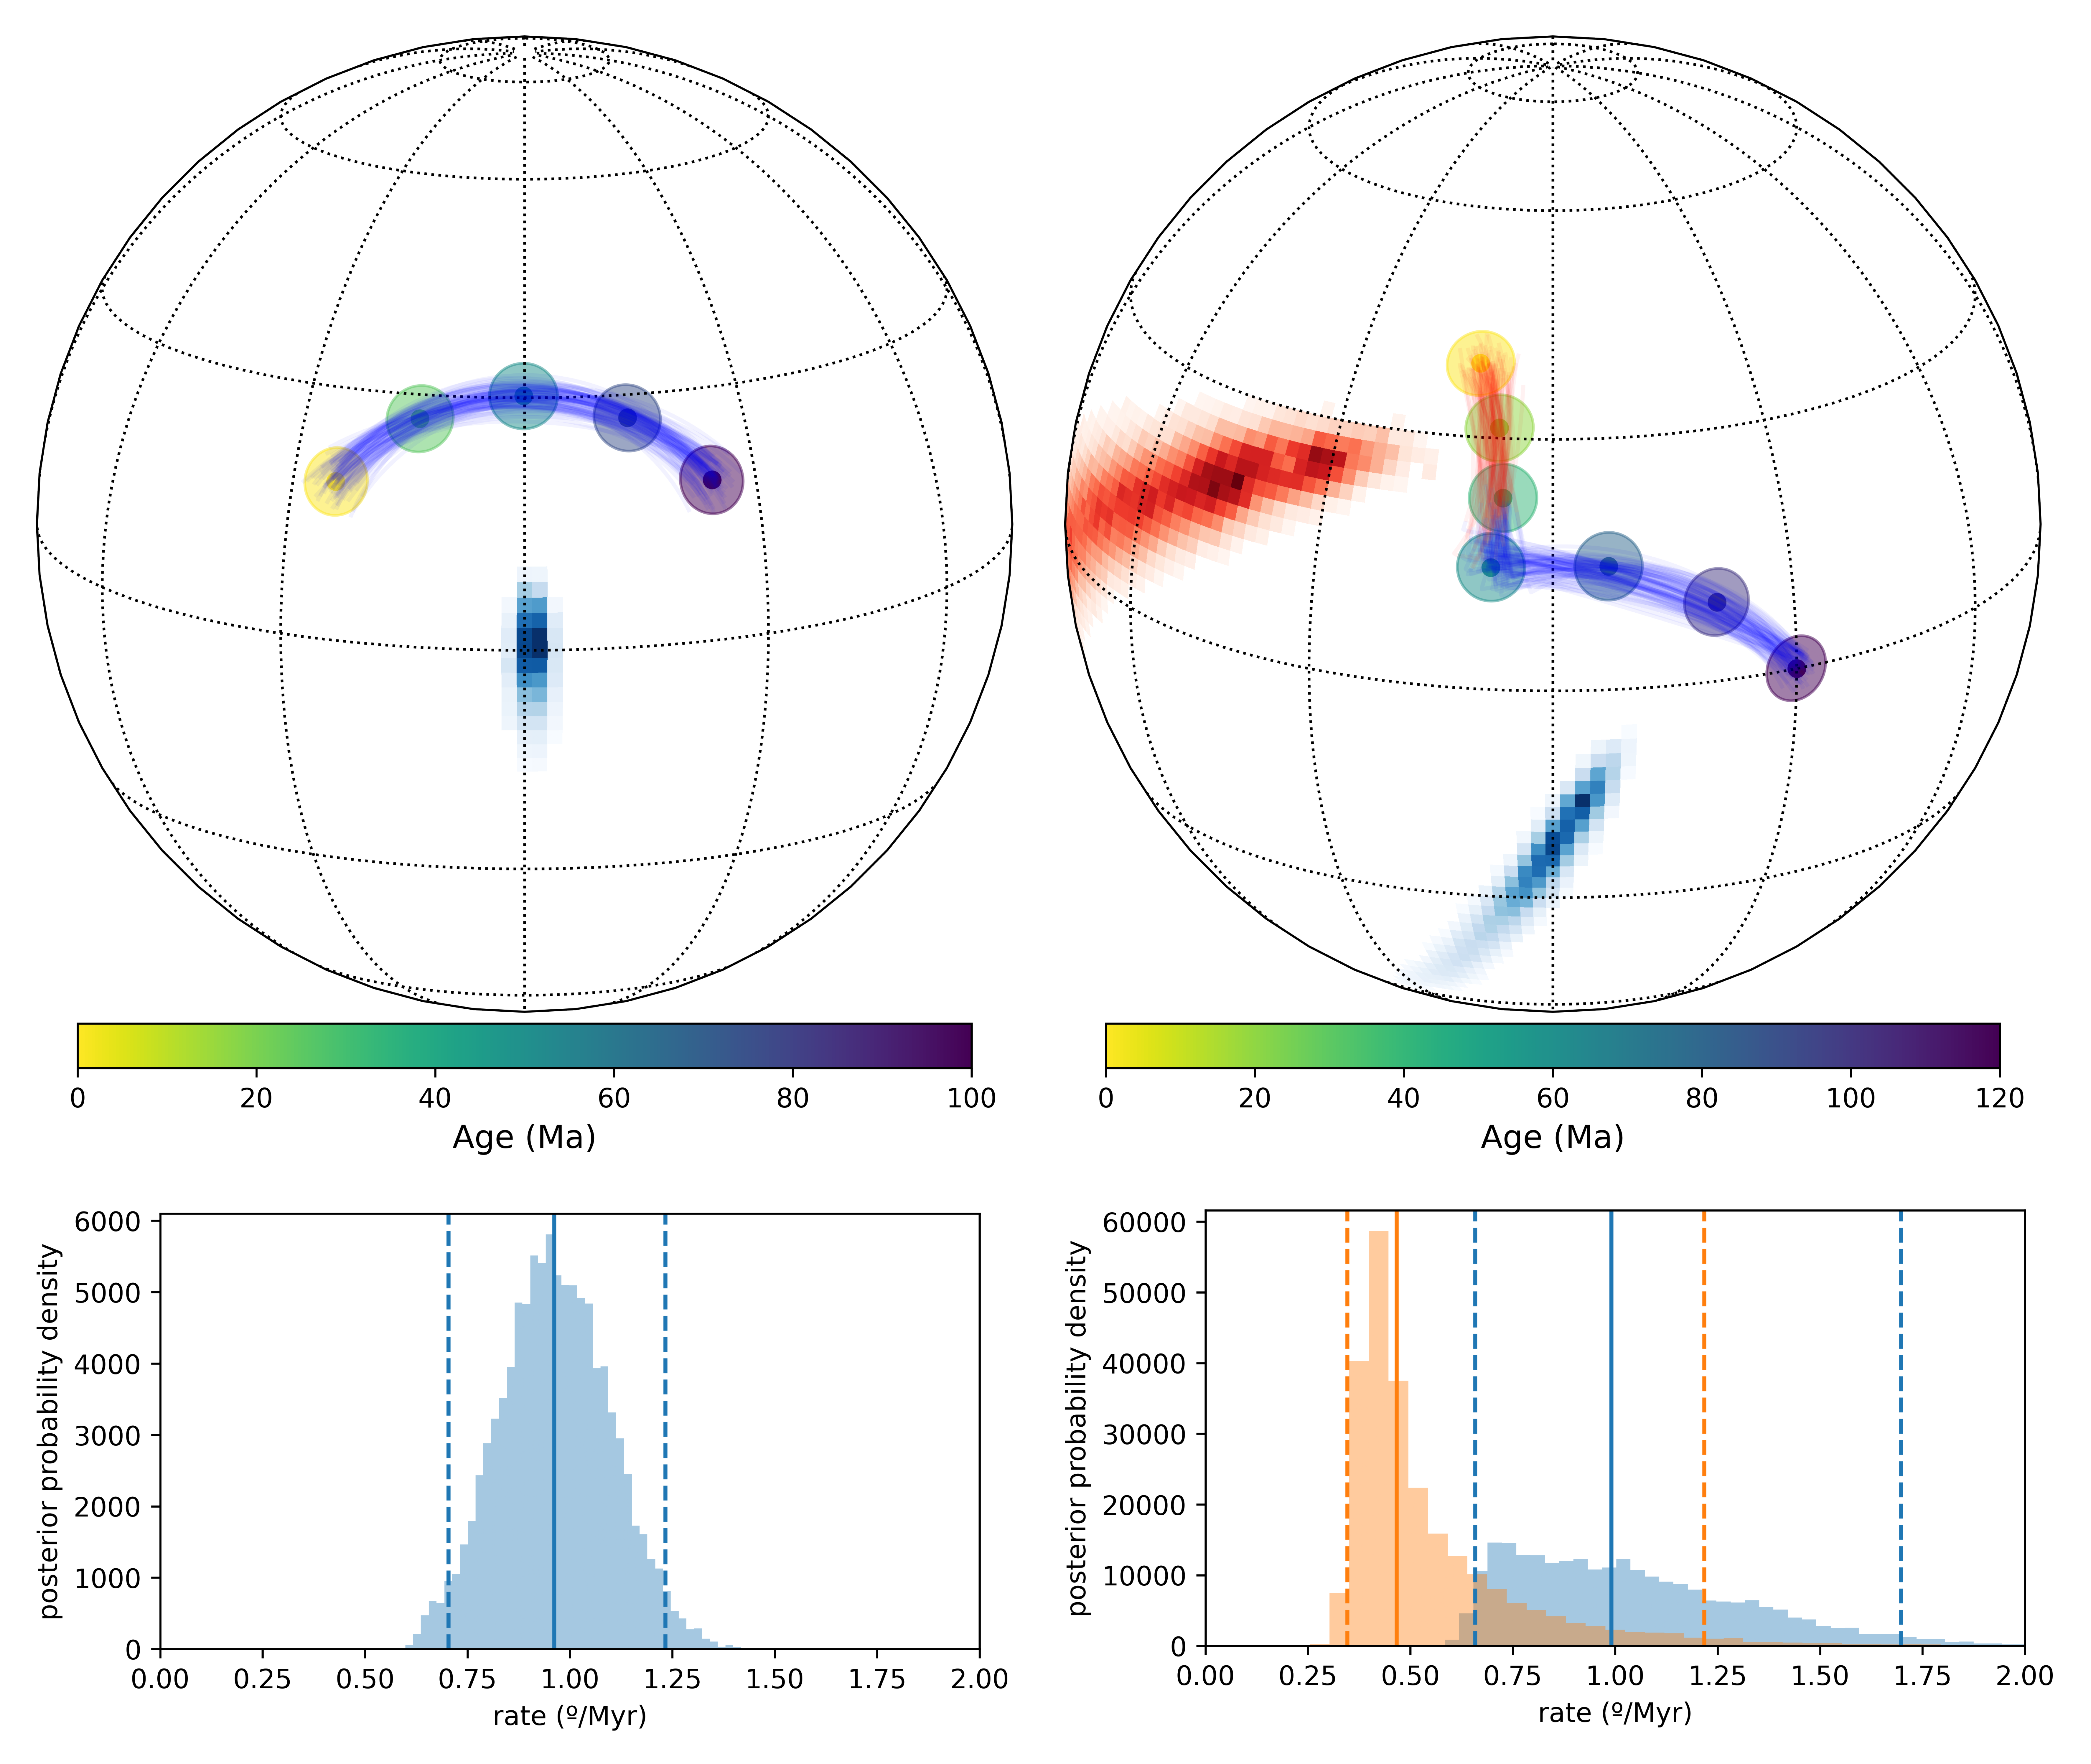
\includegraphics[width=0.9\textwidth]{fig_synthetic_pep.png}
\caption{Inversion for Euler poles from synthetic data. (A) Five paleomagnetic poles are generated during a net $100^\circ$ rotation about an Euler pole at $00^\circ$N, $000^\circ$E over 100 Myr, for a rotation rate of $1^\circ$/Myr. The blue distribution is the probability density of Euler pole positions recovered by MCMC inversion, and the blue arcs are 100 of the resulting synthetic APWPs (sampled from 50,000). The color bar scale associated with the probability density is shown in a supporting information version of this figure (Fig. S3). Such supporting information figures are provided for every Euler pole position plot in the paper (Figs S3 to S6). (B) Posterior probability density for the rotation rate of the Euler pole recovered by the inversion. The solid line shows the median of the distribution ($0.96^\circ$/Myr), and the dashed lines show the 95\% credible interval ($0.70^\circ-1.23^\circ$/Myr). (C) Paleomagnetic poles generated using two distinct Euler poles. The first Euler pole is located at $10^\circ$S, $000^\circ$E (blue star), and rotates at $1.5^\circ$/Myr for 60 Myr. The second Euler pole is located at $10^\circ$N, $300^\circ$E (red star), and rotates at $0.75^\circ$/Myr for 60 Myr. The blue and red distributions show the posterior estimate location of the first and second Euler poles (respectively) recovered by the MCMC inversion. The blue and red arcs are 100 of the synthetic APWPs. (D) Posterior probability density for the rotation rates of the Euler poles recovered by the inversion. The solid lines show the median values of the distributions ($\sim1.45^\circ$/Myr and 0.76$^\circ$/Myr for Euler rotation 1 and 2), and the dashed lines show the 95\% credible intervals.}
\label{fig:synthetic_pep}
\end{figure*}

\subsection{Two Euler rotations}
\label{sec:two_stage_poles}
We next consider an inversion for an APWP with two stage poles. Unlike the previous example where we inverted for a single Euler pole, this inversion also requires a changepoint. We generate nine idealized paleomagnetic poles with A$_{95}$ of $4^\circ$ for each from a starting point at $5^\circ$S, $030^\circ$E. The first rotation is around an Euler pole at $10^\circ$S, $000^\circ$E, and rotates at $1.5^\circ$/Myr for 60 Myr. The second rotation is around an Euler pole at $10^\circ$N, $300^\circ$E and rotates at a rate of $0.75^\circ$/Myr for the same amount of time. The synthetic poles associated with this two stage model are shown in Figure \ref{fig:synthetic_pep}. 

During the inversion, the prior knowledge for the Euler rotation axes and rates and the age of the paleomagnetic poles are set in the same way as in the one Euler rotation section above. The prior distribution for the changepoint is set as a uniform distribution with the minimum and maximum ages being the age of the youngest and oldest paleomagnetic poles. 

The inversion successfully recovers the Euler pole rotation rates with posterior distributions centered near the true values. The inversion also successfully recovers the changepoint of 60 Ma between the first and second Euler pole with a 95$\%$ credible interval for the changepoint of 65 to 55 Ma.  The inverted Euler pole positions for the first stage pole (blue distributions in Fig. \ref{fig:synthetic_pep}C) are centered near the true location (blue star in Fig. \ref{fig:synthetic_pep}C) and the inverted second Euler pole positions (red distributions in Fig. \ref{fig:synthetic_pep}C) encompass the true location as well (red star in Fig. \ref{fig:synthetic_pep}C). There is a larger spread in credible Euler pole positions for the second Euler pole particularly in the direction perpendicular to the APWP. The greater uncertainty on the location of the second Euler pole results from the motion along the APWP being smaller relative to the uncertainty on the paleomagnetic pole positions. As a result, the inverted paths have more variable curvature.  

Overall, this example demonstrates that the inversion framework can resolve APWPs with more than one stage pole and provides posterior probability distributions on the Euler rotation changepoint in addition to the multiple Euler poles positions and rates (Fig. \ref{fig:synthetic_pep}C,D).

\subsection{Incorporating age uncertainty}
\label{sec:age_uncertainty}
A benefit of the Bayesian approach to inverse problems is its generality. As long as some effect can be described statistically and incorporated into our forward model, we can include it in the inverse problem. As a result, we are able to include uncertainties on the ages of paleomagnetic poles. Assigning a fixed single age to paleomagnetic poles can bias an analysis when the age of a pole is not precisely known. The inversion framework enables the varying certainty on pole ages to be incorporated into the analysis. To demonstrate this capability, we use a similar test case as in the one Euler pole inversion with the ages of synthetic poles being adjusted to span from 140 Ma to 40 Ma (poles of 140, 115, 90, 65, and 40 Ma) (Fig. \ref{fig:age_uncertainty_samples}A), but assign prior distributions for the ages of the poles. For the first and last poles, we assume they are radiometrically dated with standard deviations of 5 Myr. However, we assume that the middle three poles have no age control, except that their ages are constrained to be between the first and last poles. We thus assign Gaussian prior distributions to the first and last poles and uniform prior distributions to the middle three (Fig. \ref{fig:age_uncertainty_samples}B). Despite this uninformative prior distribution on the age of the middle three poles, the inversion successfully places the estimated distributions of ages of the middle three poles to be centered at \textit{ca.} 115 Ma, \textit{ca.} 90 Ma,  and \textit{ca.} 65 Ma as can be seen in their posterior age distributions (Fig. \ref{fig:age_uncertainty_samples}D).

For real data, adding uncertainties to the ages of the poles enables us to properly represent our knowledge of the constraints on the APWP. These uncertainties enable data to constrain the location of the path without providing an overly tight constraint on the timing when the true age is uncertain. The resulting posterior distributions provide predicted ages for the poles associated with Euler pole inversions (Fig. \ref{fig:age_uncertainty_samples}D).

\begin{figure*}
\centering
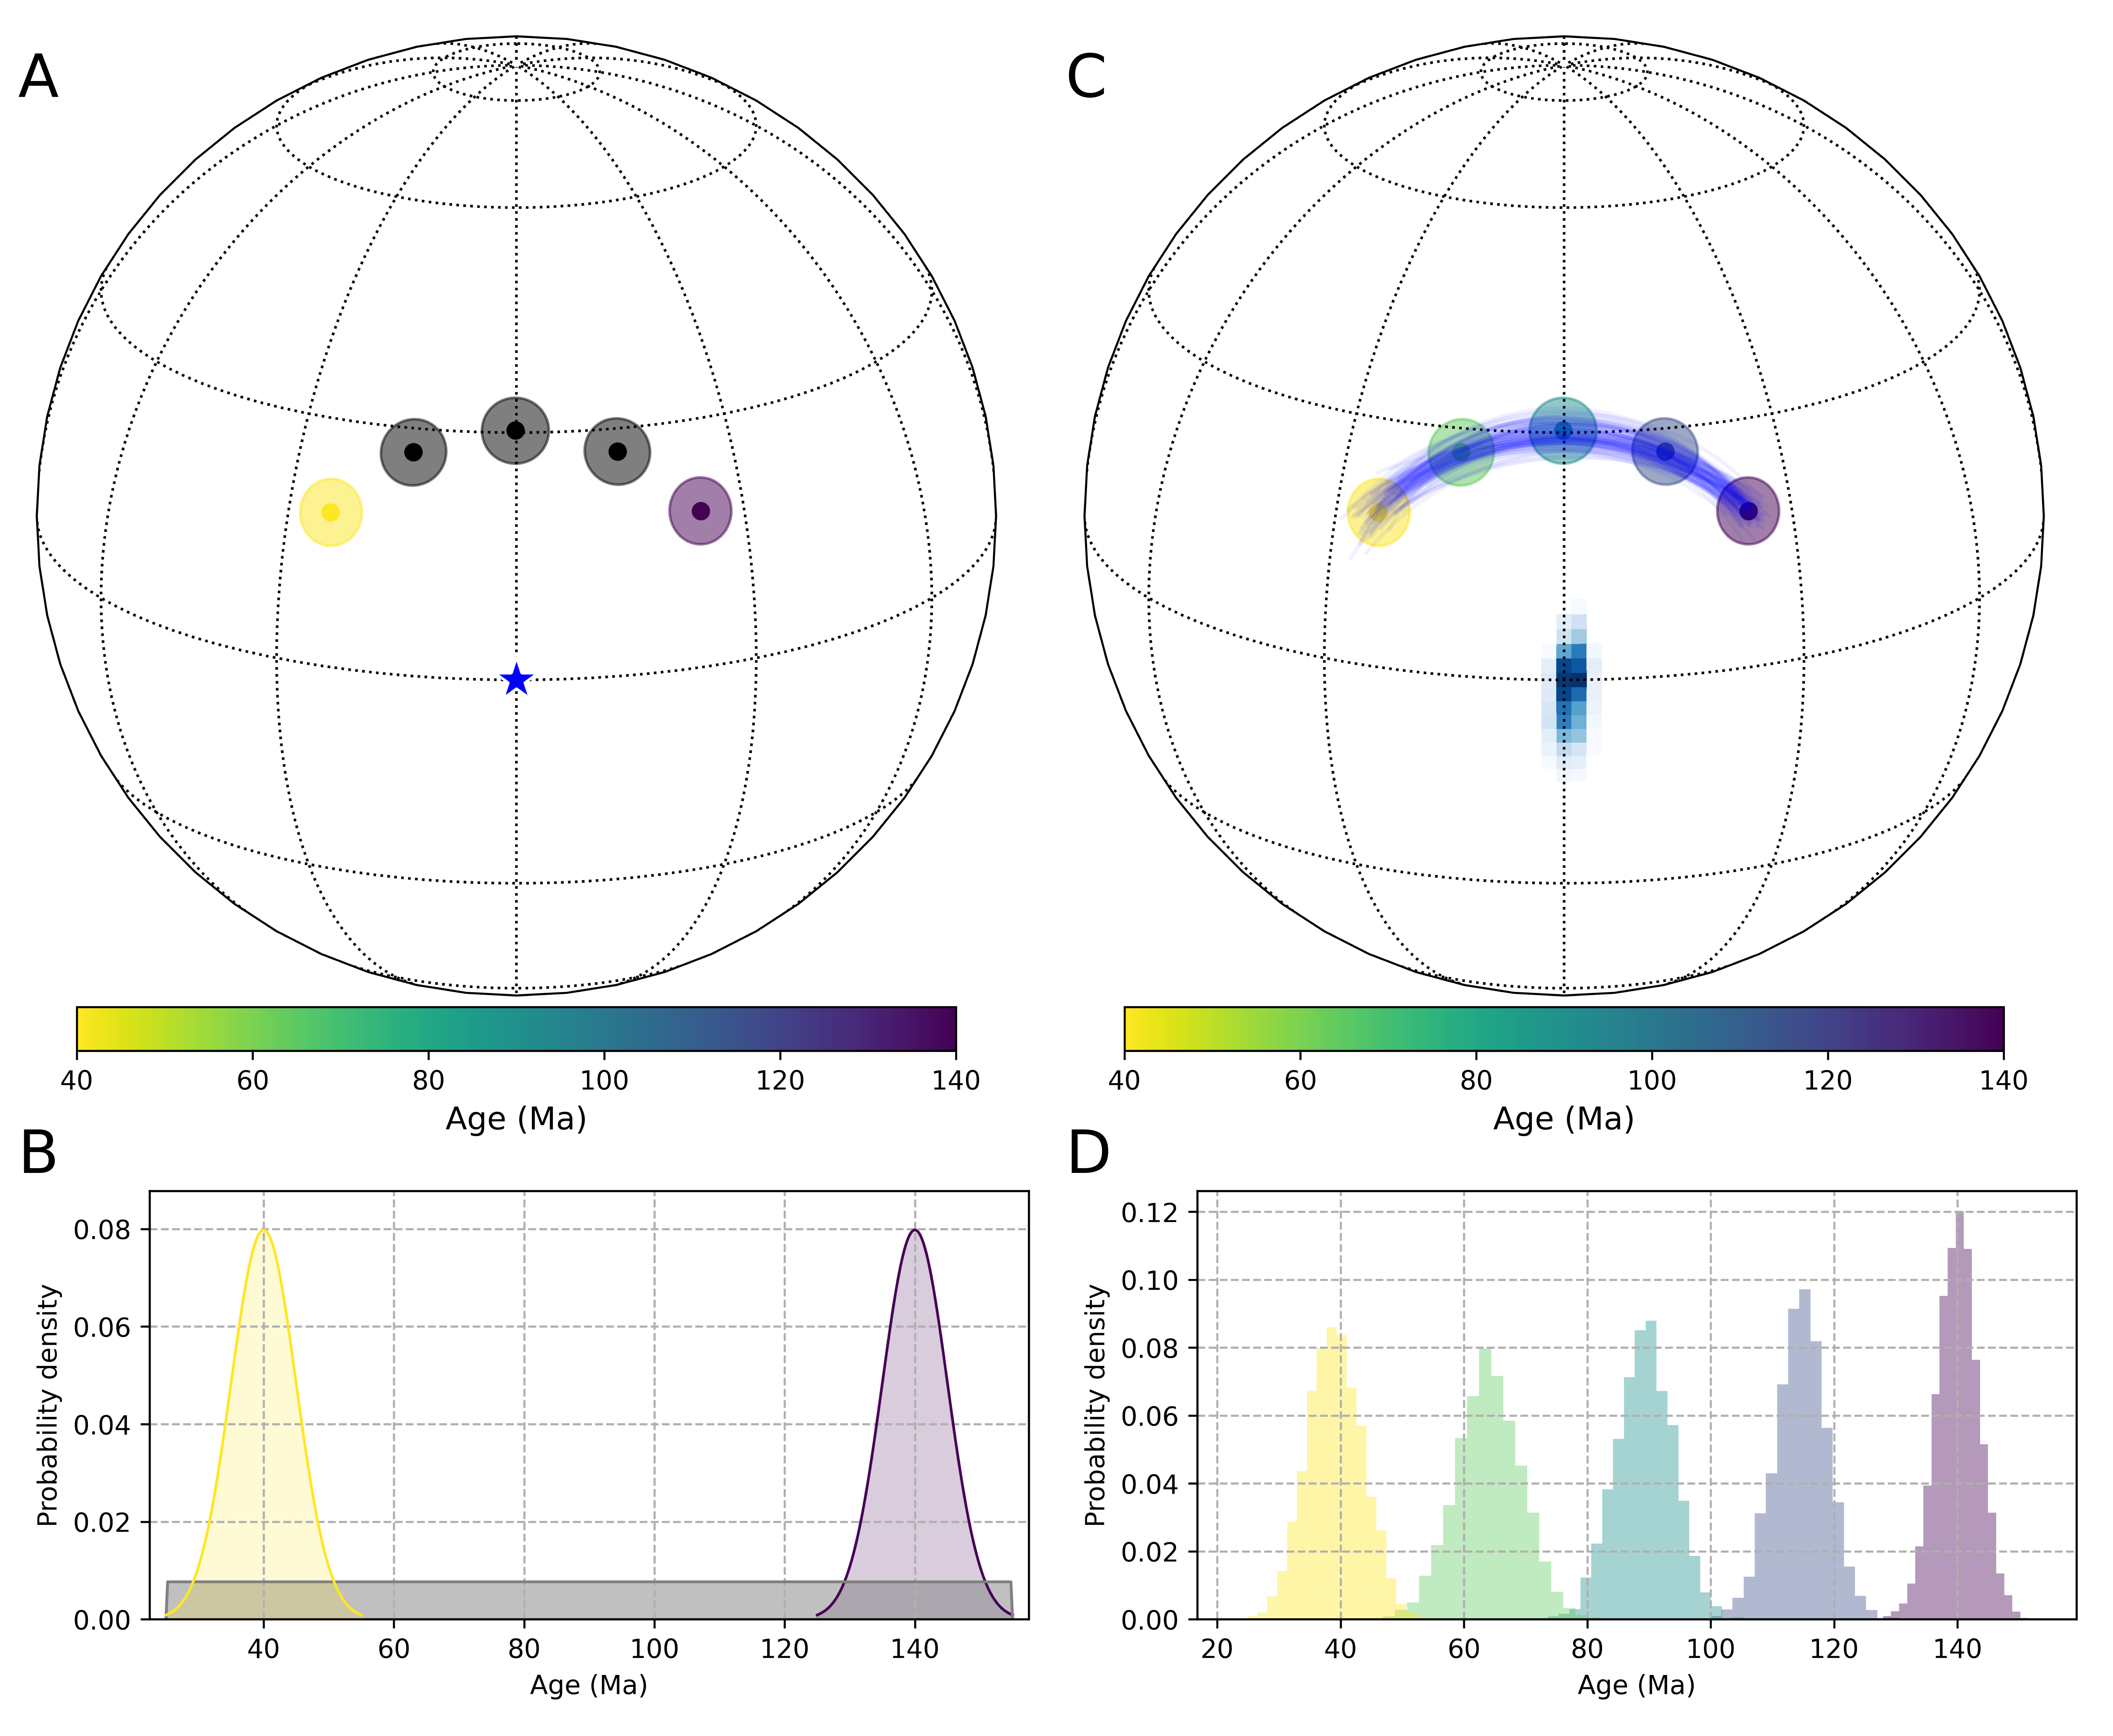
\includegraphics[width=0.9\textwidth]{fig_inversion_with_age_uncertainties.png}
\caption{Synthetic data and one Euler pole inversion incorporating age uncertainty. (A, B) Assigned distributions associated with the paleomagnetic pole positions and ages. We take the first and last poles to be radiometrically dated with 1$\sigma$ uncertainties of 5 Myr such that they are assigned Gaussian prior distributions. The middle three poles are undated and constrained to be between the first and last poles with uniform probability. (C, D) Posterior distributions after 10$^4$ MCMC samples of the Euler pole position and pole ages. The posterior distributions for the age of the middle three poles are centered on their true values of 115 Ma, 90 Ma, and 65 Ma. The middle poles help constrain the location of the Euler pole, but with their wide uniform prior age distributions do little to constrain the rotation rate.}
\label{fig:age_uncertainty_samples}
\end{figure*}

\subsection{Reporting the apparent polar wander path}
\label{sec:age_uncertainty}
A difficulty with the Bayesian approach is that the credible interval of Euler pole posterior positions are not easy to report as they do not neatly correspond to a parametric statistical distribution. We visualize the solutions with spatial histograms for the Euler pole positions and by showing example inverted paths. A typical product that one is seeking with such an inversion is an apparent polar wander path reported as interpreted pole position at given intervals. An approach that can be taken is to calculate a number of predicted pole positions at a given time implied by inverted Euler pole models and then to calculate the Fisher mean of these inverted pole positions as was done in \citeA{Swanson-Hysell2019a}. This approach provides the mean pole position on the apparent polar wander path. We also wish to report the uncertainty on that estimated position. The spread in the position of these inverted pole positions has real meaning related to the certainty of the path position at a given time resulting from the Euler pole positions and rotation rates in the posterior distribution. The spread in pole positions can be approximated as a Fisher distribution from which the angle from the mean that contains 95$\%$ of the solutions ($\theta_{95}$) can be calculated:
\begin{equation}
\theta_{95}=\frac{140^{\circ}}{\sqrt{\kappa}}
\label{eq:angular_deviation}
\end{equation}
This angle is analogous to a 2$\sigma$ uncertainty in Gaussian statistics.  The pole positions typically are consistent with being drawn from a Fisher distribution such that reporting the 95$\%$ confidence of angular deviation can be appropriate, but note that the distributions are not necessarily Fisherian such that this can be a simplified approximation. Regardless, implied pole positions from these inversions are more tightly clustered than the inverted Euler pole positions themselves. This approach for summarizing an APWP is applied to Australia's Cenozoic path in the following section.

\section{Application to Australia's Cenozoic APWP}
\label{sec:australia}

\begin{sidewaystable}[]
\scriptsize
\begin{tabular}{p{2.5 cm}lllllp{2.5 cm}lllp{3 cm}l}
\hline
Study/Region & Rock type & PLat & PLon & A$_{95}$ & N   & Pmag reference & Age (Ma) & Age min & Age max & Age information & Dist type \\
\hline
Holocene lake sediments          & sedimentary & 89.4 & 144.6 & 1.5 & 57  & \citeA{Idnurm1985a}                & 0.005      & 0        & 0.01     & radiocarbon dates from \citeA{Idnurm1985a}                                    & uniform           \\
Plio-Pleistocene mean            & mixed       & 87.7 & 353   & 3.2 & 48  & as in \citeA{Hansma2019a} & 2          & 1        & 3                 & as compiled in \citeA{Hansma2019a}                                            & uniform           \\
Glenample Fm./Port Campbell Lst. & sedimentary & 77.2 & 303.5 & 3.9 & 30  & \citeA{Idnurm1985a}                & 13         & 9        & 17       & biostratigraphy from \citeA{Dickinson2002a}                                   & uniform           \\
Cosgrove leucitite lavas         & igneous     & 80.2 & 275.4 & 8.6 & 15  & \citeA{Hansma2018a}                & 16         & 15       & 17       & Ar-Ar dates with range assigned by \citeA{Hansma2018a}                        & uniform           \\
Main Range Volcano               & igneous     & 76.6 & 271.6 & 6.1 & 25  & as in \citeA{Hansma2019a} & 23.45      & 20.2     & 26.7              & Ar-Ar dates from \citeA{Knesel2008a}                                          & uniform           \\
Tweed Volcano                    & igneous     & 77.4 & 306.9 & 5.4 & 48  & as in \citeA{Hansma2019a} & 23.9       & 23.1     & 24.7              & Ar-Ar dates from \citeA{Knesel2008a}                                          & uniform           \\
Pt. Addis Limestone              & sedimentary & 68.5 & 299.4 & 4.8 & 4.8 & \citeA{Idnurm1985a}                & 25.1       & 22.4     & 27.8     & Ar-Ar and biostratigraphic constraints from \citeA{Idnurm1985a, McLaren2009b} & uniform           \\
Springsure Volcano               & igneous     & 70.5 & 300.6 & 9.7 & 18  & \citeA{Hansma2019a}                & 28.1       & 27.8     & 28.4     & Ar-Ar date from \citeA{Cohen2013a}                                            & normal          \\
Peak Range                       & igneous     & 64.6 & 291.8 & 8.8 & 29  & \citeA{Hansma2019a}                & 29.65      & 28.2     & 31.1     & Ar-Ar dates from \citeA{Cohen2013a}                                           & uniform           \\
Hillsborough Volcano             & igneous     & 67.1 & 301.4 & 7.1 & 14  & \citeA{Hansma2019a}                & 33.6       & 33.1     & 34.1     & Ar-Ar date from \citeA{Cohen2013a}                                            & normal          \\
Browns Creek Formation           & sedimentary & 65.5 & 292.5 & 2.5 & 33  & \citeA{Idnurm1994a}                & 35.5       & 36.2     & 34.9     & biostratigraphy and magnetostratigraphy from \citeA{Shafik1997a}              & uniform           \\
North Rankin 1 Drill- core       & sedimentary & 61.7 & 298.4 & 5.1 & 20  & \citeA{Idnurm1985a}                & 59.75      & 57       & 62.5     & foraminiferal zones P3 and P4 (ages of 62.5 to 57 in GTS 2020)               & uniform        
\end{tabular}
\label{tab:Aus_Cenozoic_poles}
\caption{Paleomagnetic poles and age constraints used for the Australia Cenozoic APWP inversion and associated references. PLat = pole latitude; PLon = pole longitude; A$_{95}$ = 95\% angular confidence bounds on pole positions; N = number of site level VGPs used to calculate the mean pole positions; Pmag reference = reference for paleomagnetic pole data; Age (Ma) = nominal age calculated from age constraints on paleomagnetic poles; Age min = lower bounds for pole ages; Age max = upper bounds for pole ages; Age information = summary description for geochronology methods for pole ages and associated references;  Dist type = choice of using uniform or normal distributions for assigning prior uncertainties for pole ages.}
\end{sidewaystable}

Australia and East Antarctica were connected from the Proterozoic Eon until the Mesozoic Era when rifting led to the onset of seafloor spreading between the continents ca. 83 Ma \cite{Williams2011a, Veevers2012a}. Australia's plate motion relative to East Antarctica is considered to be well constrained from ca. 61 Ma to the present on the basis of fracture zones and magnetic anomaly data \cite{Cande2004a}. The plate motion model of \citeA{Muller2016a} utilizes the reconstruction of Australia relative to East Antarctica of \citeA{Cande2004a} for 38 Ma to the present-day and that of \citeA{Whittaker2007a} for 100 to 38 Ma. The absolute motion of Australia is constrained in the model through a plate circuit that reconstructs Australia relative to East Antarctica, East Antarctica relative to Africa, and Africa relative to the spin axis \cite{Muller2016a}. The relative motions between the plates in this plate circuit that are implemented in the plate model of \citeA{Torsvik2017a} have small differences from that of \citeA{Muller2016a} such as the use of \citeA{Tikku2000a} for the Australia to East Antarctica rotation between 84 and 44 Ma. Despite these small differences, the overall relative motions are quite similar. A more significant difference is the use of a different reference frame for the solid Earth relative to spin axis between \citeA{Muller2016a} and \citeA{Torsvik2017a}. The choice in this regard is important as pertains to comparisons with paleomagnetic data as paleomagnetic data is in the reference frame of the spin axis. The model of \citeA{Muller2016a} reconstructs plates relative to the global moving hotspot reference frame of \citeA{Torsvik2008a} which is taken as fixed relative to the spin axis over the Cenozoic. In contrast, \citeA{Torsvik2017a} utilize the global moving hotspot reference frame of \citeA{Doubrovine2012a} which includes true polar wander rotation between that reference frame and the spin axis. Notably, a recent analysis of interpreted hotspot tracks in Eastern Australia by \citeA{Hansma2020a} argued that their position in a paleomagnetic reference frame is consistent with the true polar wander implemented in the \citeA{Doubrovine2012a} reference frame. In Figure \ref{fig:Aus_Cenozoic_track}, we show the implied pole position for Australia that results from these global plate motion models. Both models imply faster Euler rotation rates after $\sim$35 Ma than before that time associated with an acceleration in Australia's northward drift (Fig. \ref{fig:Aus_Cenozoic_track}D). We use these plate motion models that are largely based on seafloor data as a comparison to an inversion of Cenozoic paleomagnetic data from Australia for the past 60 million years.

\begin{figure*}
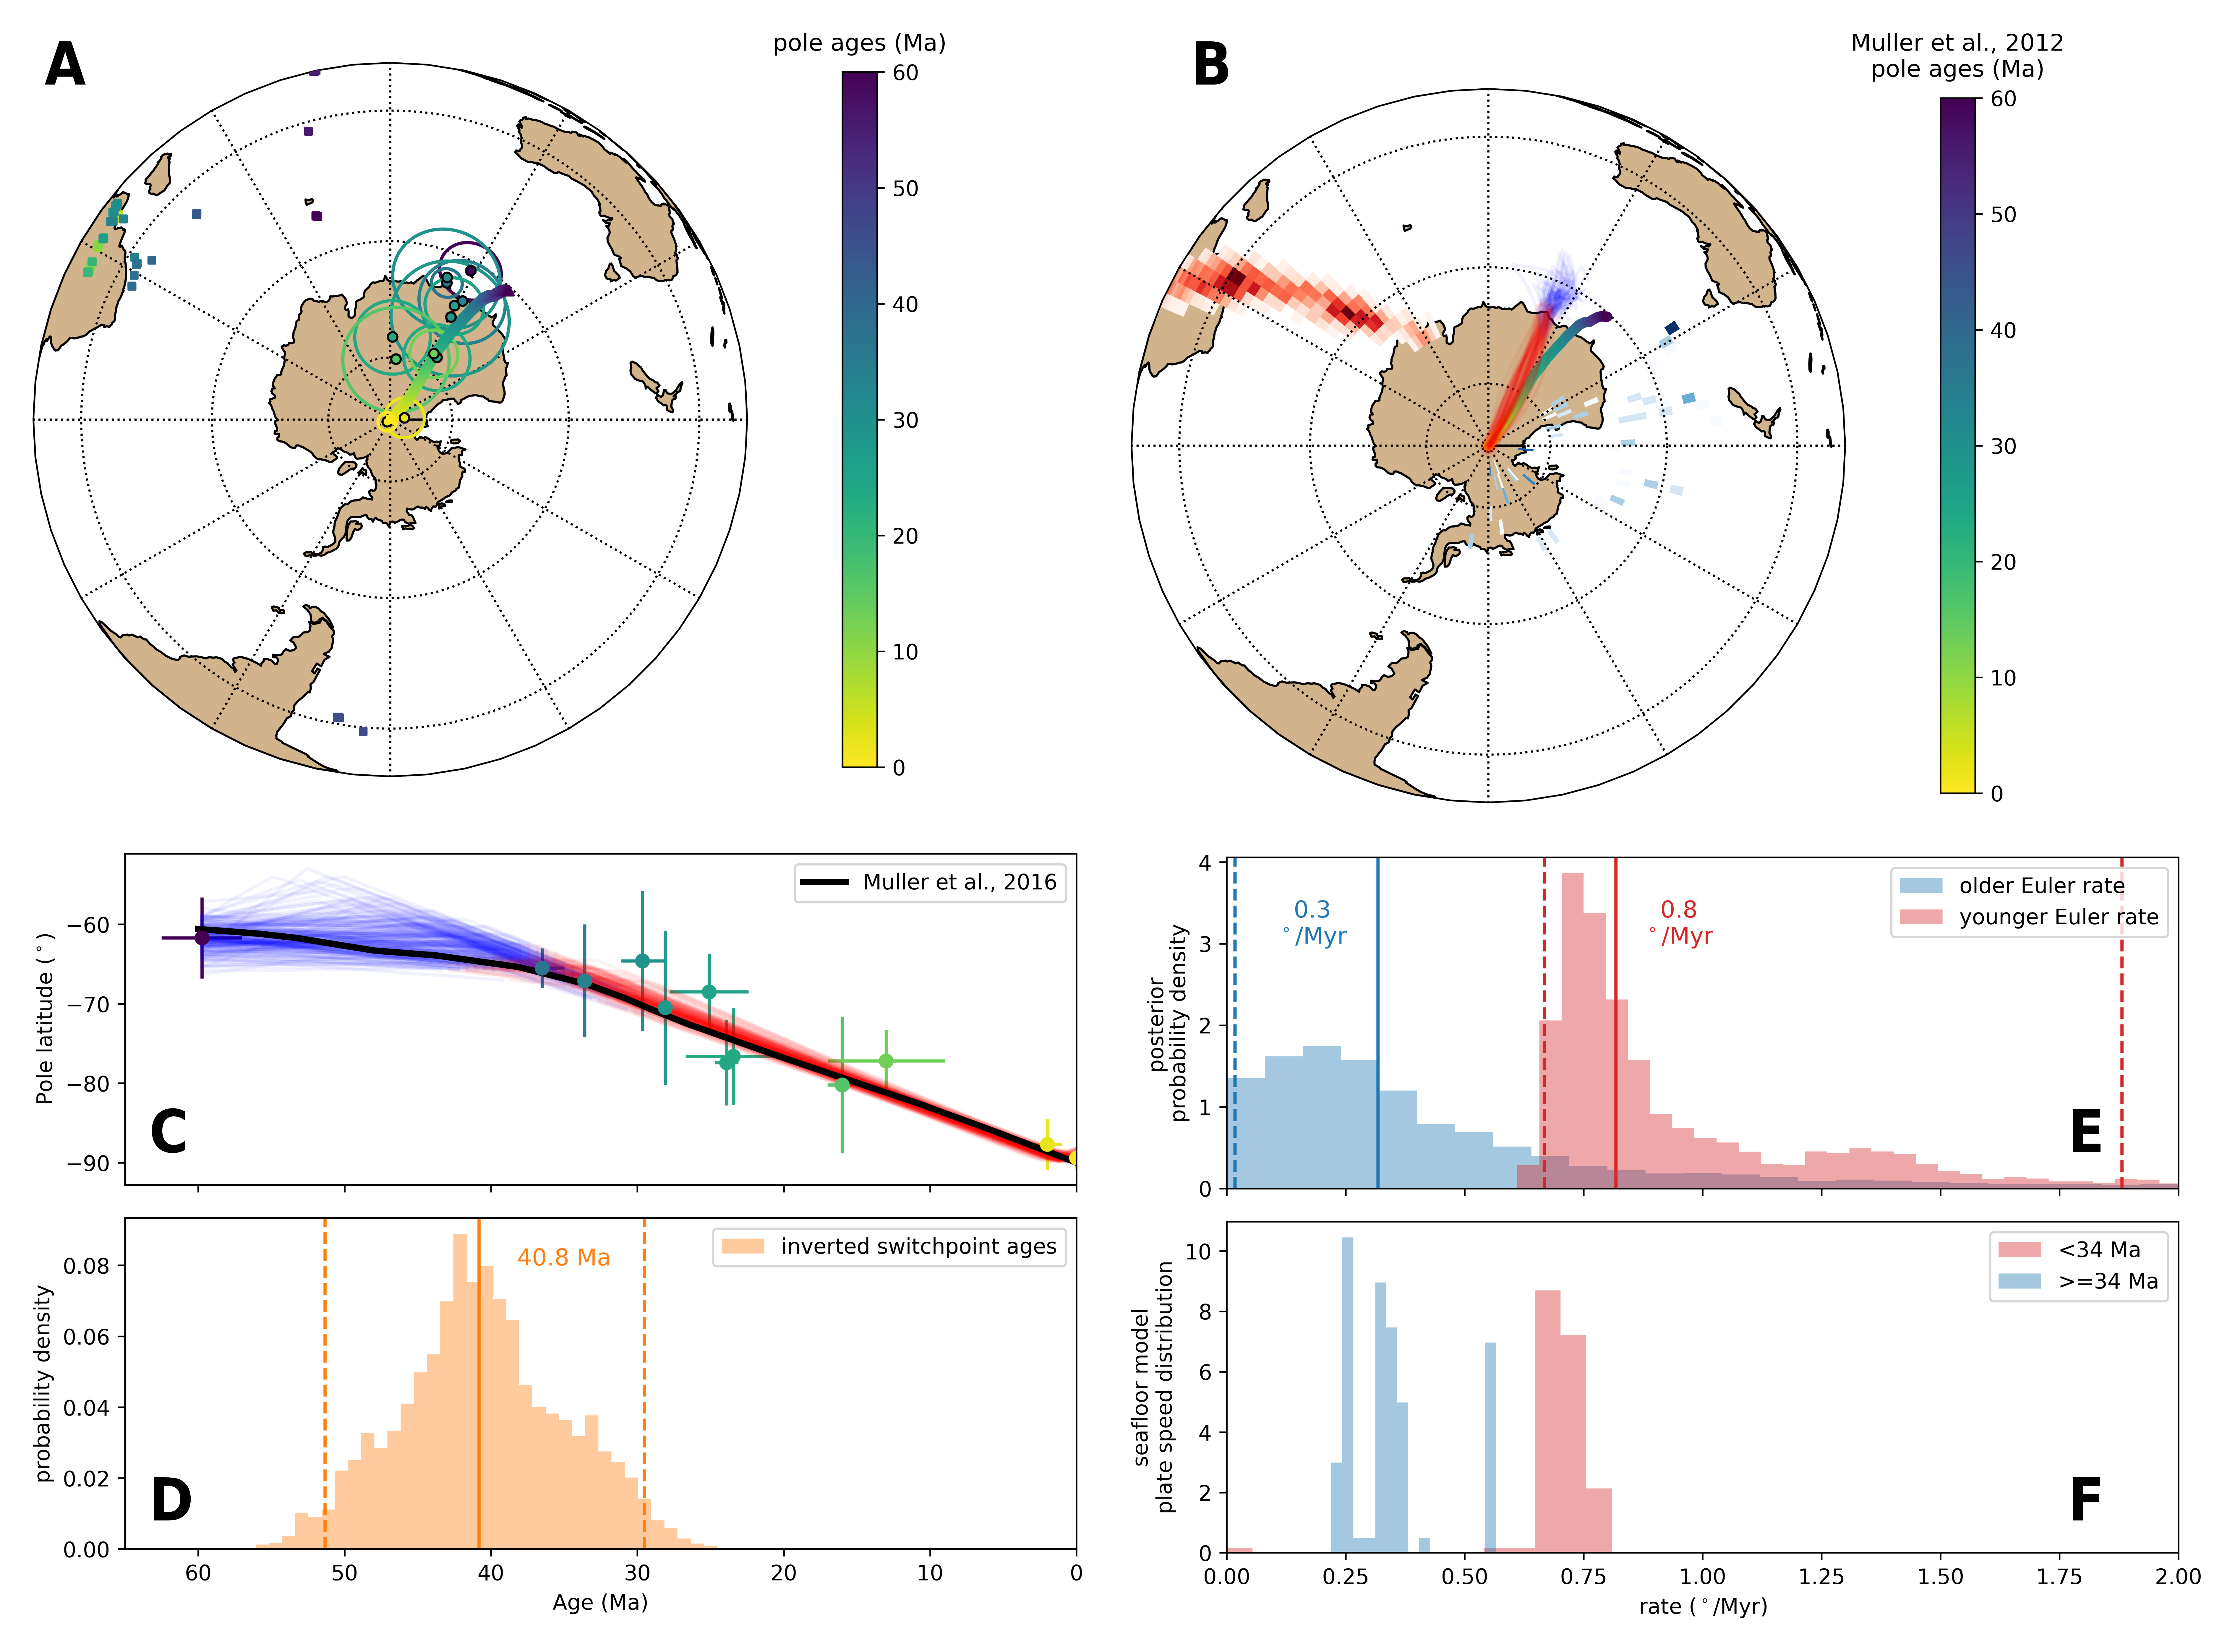
\includegraphics[width=0.9\textwidth]{fig_aus_inversion.png}
\caption{A) Cenozoic paleomagnetic poles for Australia used for the Bayesian inversion model are shown as circles with their A$_{95}$ confidence ellipses colored by age. The continuous path using the same color scale is the implied pole position extracted from the \citeA{Muller2016a} and \citeA{Torsvik2017a} models which are dominantly based on seafloor data for this time interval. B) The latitude of the pole position for the paleomagnetic poles is shown with their positional and temporal uncertainties. The black lines are the latitude of the pole position implied by the \citeA{Muller2016a} and \citeA{Torsvik2017a} models which undergo changes in slope ca. 40 to 35 Ma. The thin red and blue lines are 100 of the pole paths resulting from the two Euler pole inversion with blue being the older path segment and red the younger segment. The lower histogram shows the posterior distribution of the age of changepoints from the older to younger Euler pole in the inversion which has a median of 40.8 Ma. C) 100 sample paths (blue older; red younger) from the inversion are shown in comparison to the \citeA{Muller2016a} (triangles) and \citeA{Torsvik2017a} (squares) paths as well as density of the two inverted Euler poles (blue and red rectangles). Due to the low number of paleomagnetic poles between 60 Ma and the changepoint, as well as the short length of the path, the position of the older Euler pole is not tightly constrained leading to the sparse blue density. The posterior distribution of the younger Euler pole position (red density on the globe) is more tightly constrained and coincides with the Euler poles (red stars) extracted from the global plate reconstruction models. D) The top panel shows the posterior distribution of the Euler rotation rates associated with the older and younger inverted Euler poles with the median shown with the solid line and the labeled rates. The lower panel is the Euler rotation rates for Australia extracted from the \citeA{Muller2016a} global plate reconstruction model before and after 38 Ma illustrating good correspondence between the median of the inversion posterior and the rates from this seafloor data based model.}
\label{fig:Aus_Cenozoic_track}
\end{figure*}

There is a contentious history of interpreting Australia's Cenozoic paleomagnetic record leading to varying APWPs with discussions of the relative fidelity of igneous and sedimentary poles in the literature \cite<e.g.>{Idnurm1985a, Musgrave1989a, Idnurm1994a, Hansma2019a}. The paleomagnetic pole database for Australia in the Cenozoic has improved substantially with the development of both new Oligocene and Miocene paleomagnetic data \cite{Hansma2018a, Hansma2019a} and Ar-Ar dates that provide ages for both previously undated units and supersede previous K-Ar dates \cite{Cohen2008a,Knesel2008a,Cohen2013a}. This updated paleomagnetic pole database is listed in Table 1 and visualized in Figure \ref{fig:Aus_Cenozoic_track}A. These paleomagnetic poles give us the opportunity to develop paleomagnetic Euler pole inversions that can be compared to the independent plate tectonic reconstructions of \citeA{Muller2016a} and \citeA{Torsvik2017a}. 

The paleomagnetic data necessitate at least one change in the Euler pole between 60 Ma and the present. This need for more than one Euler pole is most readily visualized in the latitude of the poles which implies a change in rate between 60 Ma and the present (Fig. \ref{fig:Aus_Cenozoic_track}B). We apply the Bayesian inversion framework to invert for two Euler poles for Cenozoic Australia using prior probability constraints from these paleomagnetic poles. We use an uninformed prior probability for the timing of the changepoint between the two Euler poles in which it is assigned a uniform probability distribution between the age of the oldest ($\sim60$ Ma) and the youngest paleomagnetic poles ($\sim0.005$ Ma) in the compilation. We also use a weakly informative uniform prior distribution of $U(0,4)$ for the Euler rotation rate, as we know based on the position and age of the paleomagnetic poles that the overall plate motion rate for Australia in the Cenozoic is most likely to be less than 4\textdegree/Myr (Fig. \ref{fig:Aus_Cenozoic_track}A). For the prior distribution for the Euler rotation axes, we use a weakly informative Watson girdle distribution with $\kappa_W$=-0.1. 

\begin{figure}
\centering
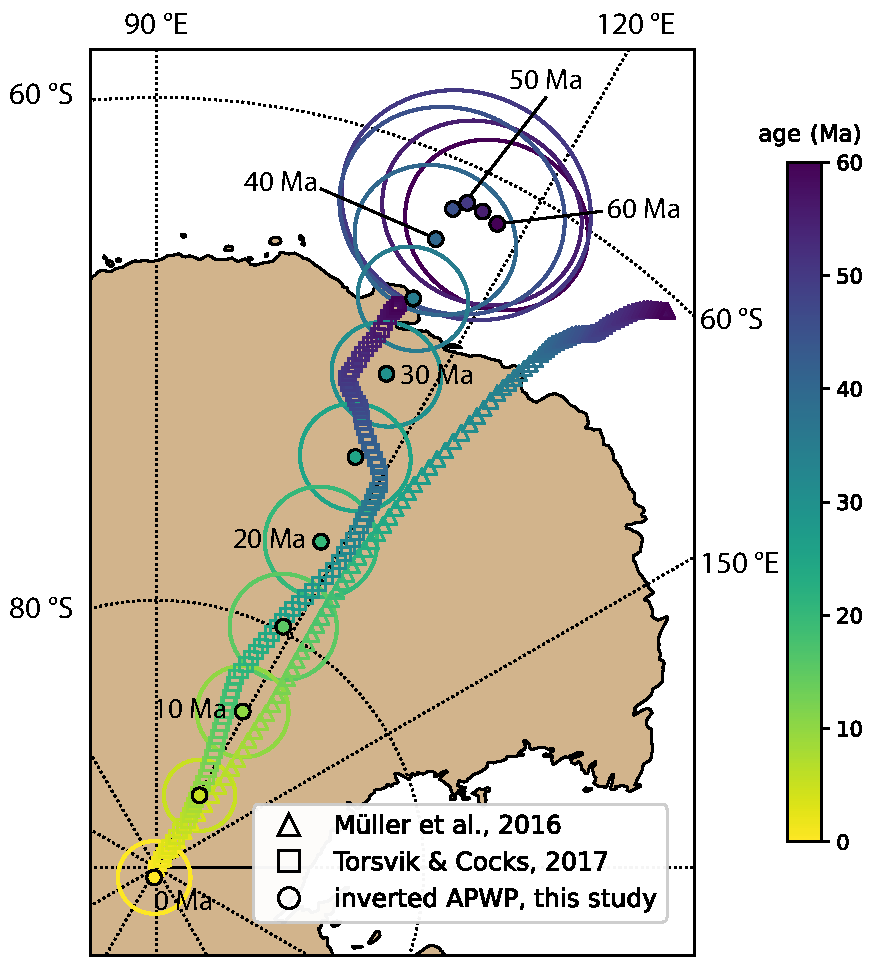
\includegraphics[width=0.5\textwidth]{fig_aus_predicted_APWP.pdf}
\caption{Summary of the apparent polar wander path (APWP) for Australia in the Cenozoic based on a two plate tectonic Euler poles Bayesian inversion to the paleomagnetic poles (Fig. \ref{fig:Aus_Cenozoic_track}). The Fisher angular deviation ($\theta_{95}$) of the positions along the inverted paths are shown in 5 Myr intervals from 60 to 0 Ma (Table \ref{tab:Aus_inverted_APWP}). Also shown are the pole positions implied by the continuous reconstructions of \citeA{Muller2016a} and \citeA{Torsvik2017a} which vary in terms of their reference frames as discussed in the text. The new inverted APWP matches better in terms of pole position latitude with the global plate reconstruction model of \citeA{Muller2016a}, but better in terms of pole position longitude with the model of \citeA{Torsvik2017a}.}
\label{fig:Aus_inverted_APWP}
\end{figure}

The posterior distribution of the Euler pole positions, samples of the small circle paths generated from the posterior distributions, the implied pole latitudes, and the full plate motion angular rotation rates are shown in Figure \ref{fig:Aus_Cenozoic_track}. The probability density of the inverted positions for the younger Euler pole (ca. 40 Ma to present) is more tightly constrained than the older Euler pole position given both the higher number of paleomagnetic poles and longer track length. The posterior distribution of the younger Euler pole positions (red density in Fig. \ref{fig:Aus_Cenozoic_track}B) recovered through the inversion correspond well with the Euler pole positions extracted from the \citeA{Muller2016a} and \citeA{Torsvik2017a} models (red and pink stars in Fig. \ref{fig:Aus_Cenozoic_track}C). The inversion is also successful in recovering the change in rate seen in both models where Australia's plate motion accelerated in the later portion of the Eocene (Fig. \ref{fig:Aus_Cenozoic_track}B). The posterior distributions for Euler rotation rates have median values that increase from 0.3$^\circ$/Myr to 0.8$^\circ$/Myr (Fig. \ref{fig:Aus_Cenozoic_track}D). The 95\% credible interval for the age of the changepoint associated with this change in rate spans from ca. 51 to 30 Ma with a median 40.8 Ma. While this broad posterior distribution reflects the sparse paleomagnetic poles constraints between 60 and 40 Ma, the timing of the change in rate is consistent with the \citeA{Muller2016a} and \citeA{Torsvik2017a} models (Fig. \ref{fig:Aus_Cenozoic_track}B). 

There is a closer correspondence between the latitude of the path inverted using the paleomagnetic pole constraints with the \citeA{Muller2016a} model than the \citeA{Torsvik2017a} model as can be seen by the inverted paths (red for younger Euler; blue for older Euler) plotting atop the thicker dashed line in Figure \ref{fig:Aus_Cenozoic_track}B. In contrast, there is a tighter correspondence between the longitude of the pole path resulting from the inversion with the \citeA{Torsvik2017a} model as seen in Figure \ref{fig:Aus_Cenozoic_track}B where the inverted paths are atop the squares which mark the \citeA{Torsvik2017a} path. The path of \citeA{Muller2016a} deviates to the east from the inverted paths whose trajectory are being constrained by the ca. 60 Ma North Rankin 1 Drillcore pole (Table 1). To facilitate these comparisons, we apply the approach described in the \textit{Reporting the apparent polar wander path} section to summarize the new APWP (Table \ref{tab:Aus_inverted_APWP}) and plot it with the implied pole positions of the \citeA{Muller2016a} and \citeA{Torsvik2017a} models in Figure \ref{fig:Aus_inverted_APWP}.

\begin{table}
\footnotesize
\caption{Bayesian paleomagnetic Euler pole apparent polar wander path for Cenozoic Australia}
\centering
\begin{tabular}{cccc}
\hline
\multicolumn{4}{c}{Bayesian PEP (2 plate tectonic Euler poles)} \\
\hline
Age (Ma)       & PLon\textdegree       & PLat\textdegree        & $\Theta_{95}$      \\
60           & 117.9       & -61.8       & 3.5                \\
55           & 116.4       & -61.6       & 3.8                \\
50           & 115.1       & -61.6       & 4.8                \\
45           & 114.2       & -62.0       & 4.3                \\
40           & 114.0       & -63.5       & 3.1                \\
35           & 114.3       & -66.1       & 2.1                \\
30           & 115.0       & -69.3       & 2.1                \\
25           & 115.9       & -72.8       & 2.1                \\
20           & 116.8       & -76.3       & 2.1                \\
15           & 117.8       & -79.8       & 2.0                \\
10           & 118.9       & -83.4       & 1.7                \\
5            & 120.8       & -86.9       & 1.3                \\
0            & 282.6       & -89.6       & 1.4        \\
\hline
\end{tabular}
\label{tab:Aus_inverted_APWP}
\\
Notes: PEP: paleomagnetic Euler pole; PLon: pole longitude; PLat: pole latitude; $\Theta_{95}$ represents the Fisher angular deviation wherein 95$\%$ of the estimated path positions lie within that angle of the mean path position assuming a Fisher distribution.
\end{table}

It is intriguing that the inclusion of the \citeA{Doubrovine2012a} true polar wander correction in the \citeA{Torsvik2017a} model results in improved correspondence in the terms of pole longitude, but more of a discrepancy with the paleomagnetic poles and their inversion in terms of latitude (Figs. \ref{fig:Aus_Cenozoic_track} and \ref{fig:Aus_inverted_APWP}). While the conclusions that can be drawn in this regard are limited given the restriction of the analysis to Australia, such comparisons could be a fruitful future direction to use for comparisons between reference frames. Overall, the analysis highlights a broad agreement in the interpretation of kinematics that results from inversion of the Cenozoic paleomagnetic poles for Australia and that which results from seafloor-based plate motion models.

\section{Application to the Keweenawan Track}
\label{sec:keweenawan}

An impetus for the development of this Bayesian paleomagnetic Euler pole inversion method was to constrain the absolute rates of plate motion associated with the ca. 1109 to 1070 Ma Keweenawan Track of paleomagnetic poles from the Proterozoic continent of Laurentia \cite{Halls1982a, Swanson-Hysell2009a, Swanson-Hysell2019a}. These poles are associated with the rapid motion of Laurentia towards the equator leading up to the Grenvillian orogeny and the assembly of the supercontinent Rodinia \cite{Swanson-Hysell2021a}. While previous approaches had established estimates for the rate of latitudinal motion associated with the Keweenawan Track \cite{Davis1997a, Swanson-Hysell2014b}, this Bayesian inversion method was implemented in \citeA{Swanson-Hysell2019a} in order to constrain absolute rates (without providing the level of detail on the methodology that is elucidated in the present contribution). In addition to our goals of constraining absolute rates, this approach was particularly appropriate for the Keweenawan Track as it includes poles with quite disparate precision on their age constraints as some are constrained tightly by high-precision U-Pb dates \cite<e.g.>{Fairchild2017a} while others have looser stratigraphic constraints. A technical note related to the analysis in \citeA{Swanson-Hysell2019a} is that it used a version of the code written in PyMC2 (\citeA{Patil2010a}; \url{https://github.com/ian-r-rose/mcplates}). The PyMC project has migrated to PyMC3 (now known simply as PyMC) which is a total rewrite of the module \cite{Salvatier2016a} and necessitated our code to refactored into its present PyMC version (\url{https://github.com/Swanson-Hysell-Group/Bayesian_PEP_inversion}). These two versions of the code apply the same methodology and recover very similar solutions. One change that we adopted in this study is that we applied inclination shallowing corrections to the sedimentary paleomagnetic poles within the Keweenawan Track (i.e. the Nonesuch Formation and lower Freda Formation poles of \citeA{Henry1977a}) given how widespread inclination shallowing is for remanence held by detrital hematite. While more research is needed on these sedimentary rocks to quantify the degree of inclination shallowing, we take the approach of \citeA{Domeier2012a} in utilizing an assumed flattening factor of 0.6 given that sample-level data are not available. A ripe direction for future work would be to adopt a probabilistic framework for inclination shallowing correction rather than an assigned single value.

\begin{figure*}
\centering
\includegraphics[width=0.7\textwidth]{fig_Keweenawan_1.pdf}
\caption{A) Bayesian paleomagnetic Euler pole inversions of the Keweenawan Track for one plate tectonic Euler pole and for one true polar wander Euler pole. The Euler pole locations and representative predicted pole positions associated with posterior Euler parameters and pole ages are shown with the observed paleomagnetic poles on the left orthographic projections. Details on the individual paleomagnetic poles used in the analysis can be found in \citeA{Swanson-Hysell2019a}. The distribution of angular rotation rates resulting from the inversions are shown in the histograms on the right. B) Posterior likelihood distributions for all models used to invert for the Keweenawan Track. The log likelihood values are calculated by taking the natural log of equation \ref{eq:model_likelihood} and show the true polar wander (TPW) inversion to have a quite low likelihood relative to the other inversions.}
\label{fig:Keweenawan_Track_1}
\end{figure*}

\begin{figure*}
\centering
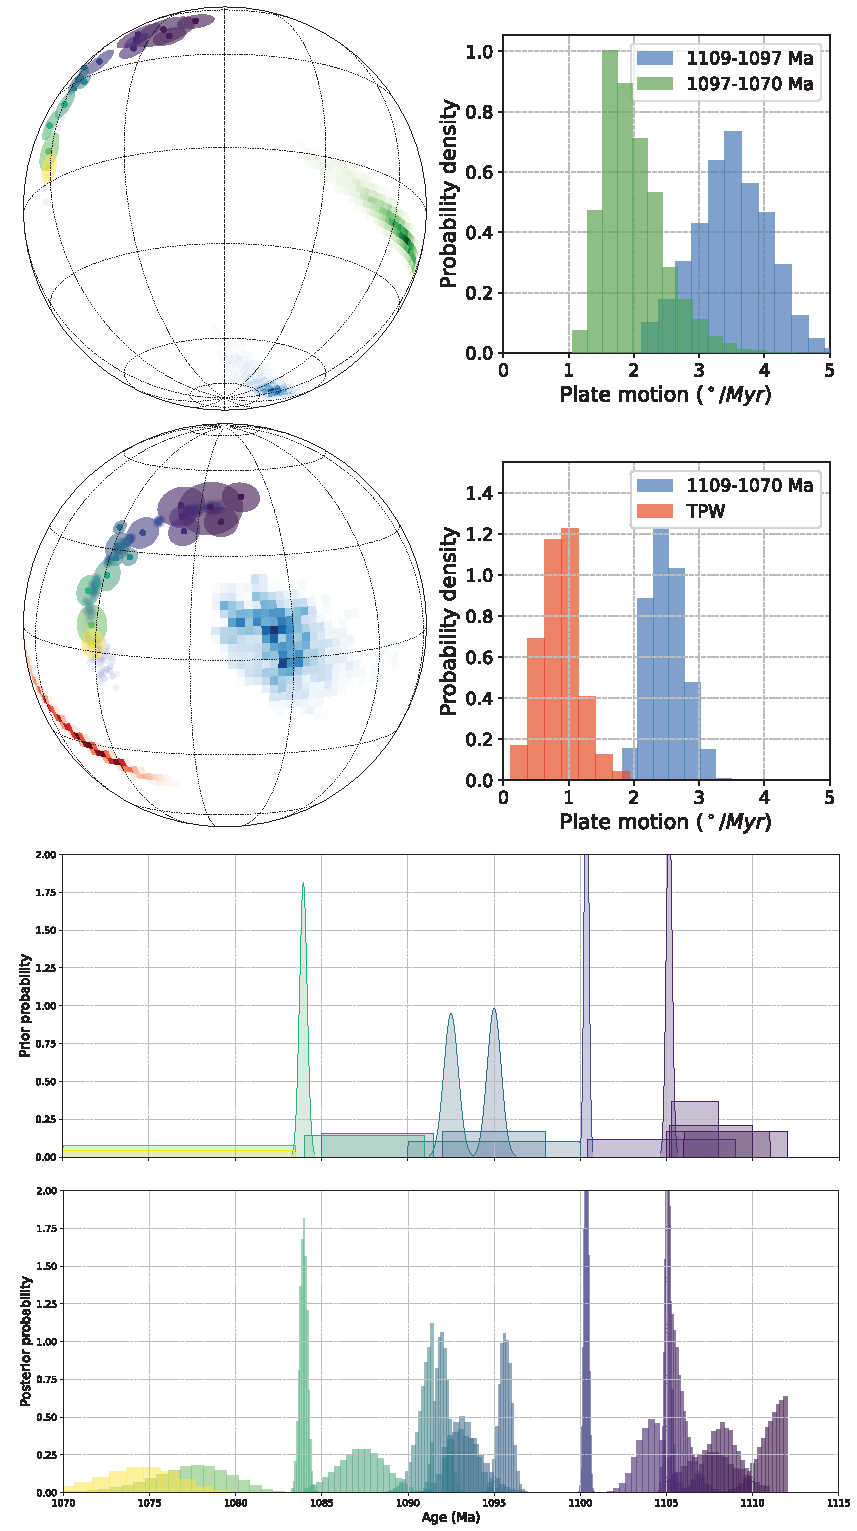
\includegraphics[width=0.7\textwidth]{fig_Keweenawan_2.pdf}
\caption{A) Bayesian paleomagnetic Euler pole inversion of the Keweenawan Track for two plate tectonic Euler poles with a change point and for one Euler pole with concurrent true polar wander. The Euler pole locations, representative predicted pole positions, and the distribution of angular rotation rates associated with each model are shown in the same way as in Fig. \ref{fig:Keweenawan_Track_1}. For the plate tectonic Euler pole, the position (in blue density) is shown relative to the start position of the path. The true polar wander rotation will progressively rotate these plate tectonic Euler poles such that the position will change through time. The log likelihood of these models are compared with others in Fig. \ref{fig:Keweenawan_Track_1}B. B) Top: prior age distributions for poles used in the forward model. Bottom: posterior pole age distributions resulting from the two plate tectonic Euler pole MCMC inversion.}
\label{fig:Keweenawan_Track_2}
\end{figure*}

For all Keweenawan Track inversions, we use weakly informative Watson girdle distributions with $\kappa_W$=-0.1 for the prior distribution of Euler poles, and use an exponential distribution with $\lambda$=2.5 for the prior distribution of Euler rotation rates (based on the analysis shown in Figure \ref{fig:euler_pole_prior}). Paleomagnetic Euler pole inversions to the Keweenawan Track are shown in Figures \ref{fig:Keweenawan_Track_1} and \ref{fig:Keweenawan_Track_2}. The posterior distribution of the Euler pole positions are shown along with a sampling of pole positions generated from the posterior Euler parameters and pole ages which are plotted over the paleomagnetic poles (as compiled in \citeA{Swanson-Hysell2019a}). The prior distributions for the ages of the poles are shown in Fig. \ref{fig:Keweenawan_Track_2}B. The prior probabilities assigned to the ages illustrate the variable age uncertainties associated with the paleomagnetic poles in the Keweenawan Track some of which are tightly constrained by radiometric dates and others which have looser age constraints \cite{Swanson-Hysell2019a}. The posterior distribution of the angular rotation rates for Laurentia resulting from the inversions are shown as angular velocities along with their 95\% credible intervals (Figs. \ref{fig:Keweenawan_Track_1} and \ref{fig:Keweenawan_Track_2}). To compare models with varying combinations of Euler poles and assess whether the results of the inversions represent good fits for the observed paleomagnetic poles, we calculate the distribution of the natural log of the likelihood for the paleomagnetic poles generated from the posterior Euler parameters and pole ages based on the observed paleomagnetic poles. A summary of the posterior likelihood distributions is shown in Fig. \ref{fig:Keweenawan_Track_1}B. 

Applying a single paleomagnetic Euler pole inversion to the entirety of the Keweenawan Track results in a median rate of 3.1 \textdegree/Myr with a 95$\%$ credible interval of 2.7 to 3.6 \textdegree/Myr (Fig. \ref{fig:Keweenawan_Track_1}). In the literature, the Keweenawan Track has variably be interpreted as being the result of fast differential plate motion \cite<e.g.>{Davis1997a} or as the result of true polar wander \cite<e.g.>{Evans2003b}. True polar wander results in rotation of the entire silicate Earth about an Euler pole 90$^\circ$ from the path and has the potential to progress at rapid rates \cite{Rose2017b}. Overall, true polar wander is a difficult signal to disentangle from plate motions, since any given APWP can be the result of true polar wander, plate tectonics, or some combination of the two. However, given the nature of a true polar wander rotation, an Euler pole that describes true polar wander will be 90$^\circ$ from the spin axis such that the Euler pole for a true polar wander event will be 90$^\circ$ from the paleomagnetic poles. Therefore, the extent to which true polar wander could explain motion of the Keweenawan Track can be evaluated by constraining the location of the true polar wander Euler pole to be within a great circle 90$^\circ$ from the path. This constraint is imposed in the inversion by using a restrictive Watson girdle distribution. As shown in \citeA{Swanson-Hysell2019a}, a single true polar wander rotation is a poor fit to the path given its curvature. The posterior true polar wander rotation parameters results in a path that deviates from the observed paleomagnetic poles, as is illustrated by the resampled poles for younger ages falling outside of the A$_95$ uncertainty ellipses of the observed paleomagnetic poles in Fig. \ref{fig:Keweenawan_Track_1}A. As a result, the posterior log likelihood values for the true polar wander model are much smaller than those for the one Euler pole model (Fig. \ref{fig:Keweenawan_Track_1}B).

The pole path could be the result of a combination of true polar wander and differential plate motion. This scenario can be explored through models that invert for a true polar wander Euler pole as well as differential plate tectonic Euler poles. The model with both a plate tectonic Euler pole rotation and a concurrent true polar wander rotation partitions the motion between both with significantly faster plate tectonic motion (Fig. \ref{fig:Keweenawan_Track_2}A). In addition, because the true polar wander involves the rotation of the solid Earth with respect to the spin axis (rotating both the plate an its associated Euler pole), its results in more uncertainty associated with the location of the plate tectonic Euler pole, broadening the posterior Euler pole distribution (Fig. \ref{fig:Keweenawan_Track_2}A). Although such a rotation is possible, adding a true polar wander component to either the one or two plate tectonic Euler pole inversions does not significantly improve fits to the observed paleomagnetic poles Figure \ref{fig:Keweenawan_Track_1}B. Overall, forward models involving small circle Euler rotations always yield better fits to the observed paleomagnetic data than the model that considers only true polar wander great circle rotation (Fig. \ref{fig:Keweenawan_Track_1}). These results indicate that there was rapid plate motion at the time which is associated with subduction that led to the closure of the Unimos Ocean leading up to collisional Grenvillian orogenesis and the associated formation of the supercontinent Rodinia \cite{Hynes2010a, Swanson-Hysell2022a}. In comparison with models that involve one Euler pole rotation, the two Euler pole inversion results in an improvement in fit as can be visualized by the modeled pole positions shown in Figure \ref{fig:Keweenawan_Track_2}A and by the calculated posterior likelihood distributions for the paleomagnetic pole positions (Fig. \ref{fig:Keweenawan_Track_1}B). The two Euler pole inversion results in a ca. 1097 Ma changepoint age (with a 95\% credible interval from 1098.8 to 1095.4 Ma) with rates that slow from $\sim$3.1\textdegree /Myr to $\sim$1.8\textdegree /Myr after the changepoint. This change could be associated with initial onset of collisional Grenvillian orogenesis along Laurentia's margin \cite{Swanson-Hysell2019a}.

The results of this Bayesian Euler pole inversion method can not only provide insights into geodynamic processes, but also provide geochronologic estimates on rock units that have poor or none radiometric age constraints. As our knowledge of paleomagnetic pole ages and their uncertainities are incorporated into the inversions, the more informative prior distributions that we implement for poles that have well-constrained radiometric dates (such as the normal distributions for many igneous units of the Keweenawan Track) can act as anchor points and result in more tightly constrained posterior distributions for ages of other poles that have less informative priors (such as the uniform distributions for some igneous and the sedimentary poles of the Keweenawan Track). As is illustrated in Figure \ref{fig:Keweenawan_Track_2}B, the poles whose ages could only be bracketed as uniform distributions in the prior end up having posterior age distributions with more constrained credible intervals. In this example, these ages estimated through paleomagnetic Euler pole inversion model give insight into the chronology of magmatism and basin development within the North American Midcontinent Rift. 

\section{Challenges and opportunities in the application of paleomagnetic Euler pole analysis}
\label{sec:challenges_and_opportunities}

While the examples in this study highlight insights that can be gained through applying paleomagnetic Euler pole analysis to segments of apparent polar wander paths, challenges remain in its broad application. One set of challenges relates to the resolving power of the method. For slow rates of motion, the position of inverted Euler poles are uncertain and it is difficult to resolve the timing of changepoints with confidence. However, this issue is more related to the precision of available constraints and is the case regardless of method. Of note is that the spread between resulting paths is much less than the spread of the posterior Euler pole position (as in the older Euler pole rotation in the Australia application; Fig. \ref{fig:Aus_Cenozoic_track}). Determining the number of change points to implement in an inversion is an additional challenge, and one that is also more difficult for slow motions or uncertain data. This issue is addressed theoretically in \citeA{Gallo2022a} who apply a frequentist approach to paleomagnetic Euler pole inversion and propose a graphical approach to evaluate for the optimal number of inverted Euler poles. The extension of such an approach beyond ideal synthetic data to noisier suites of paleomagnetic data as well as integration with our Bayesian inversion approach could prove fruitful. 

It could be interpreted as an advantage of paleomagnetic Euler pole analysis that it utilizes a physical model of plate motions to inform an APWP shape that fits with our knowledge of plate motions. However, uncertainty remains regarding underlying assumptions including that Euler pole positions and associated plate motions are relatively stable over millions of years. A complexity here is that while data constrain the relative motion between plates to be relatively constant (e.g. \citeA{Muller2016a}), the motion of a plate relative to the spin axis can be the combined effect of multiple Euler poles in a plate circuit as well as true polar wander. Furthermore, the method also assumes that the timescale over which Euler pole positions themselves migrate are relatively rapid such that they can be approximated by instantaneous changepoints. Evaluating the validity of these assumptions is an area ripe for future research. There is the potential to apply paleomagnetic Euler pole inversion itself to gain insight into these uncertainties.

An additional opportunity comes from the method giving posterior distributions for pole ages. There is a long history of paleomagnetists comparing undated (or poorly dated) paleomagnetic poles with APWPs to gain insight on their age \cite{McCabe1984b, Hnatyshin2014a}. These methods typically rely on comparison between designated pole pairs or consider the reference APWP to not have uncertainty. In the Bayesian paleomagnetic Euler pole inversion method developed here, undated poles (Fig. \ref{fig:age_uncertainty_samples}) or poorly dated poles (Fig. \ref{fig:Keweenawan_Track_2}) can be incorporated into the analysis with the resulting posterior distribution age distribution providing an estimate of the age of magnetization including uncertainty. 

\section{Conclusions}
\label{sec:conclusions}

We have extended the paleomagnetic Euler pole analysis of \citeA{Gordon1984a} by placing it within a Bayesian framework. As a Bayesian inverse problem, Markov chain Monte Carlo (MCMC) numerical methods can be used to obtain estimates of Euler pole positions and rates as constrained by paleomagnetic poles. Regularization of the inversions is not accomplished by smoothing parameters, but can instead be accomplished through prior probability distributions for the Euler pole parameters, which have clear physical interpretations. The approach enables uncertainties on both the positions and ages of paleomagnetic poles to be incorporated into the analysis. Multiple Euler poles can be included with the timing of changepoints between them being solved as part of the inversion. An advantage of this approach is that the paleomagnetic Euler poles provide an estimate for the total plate velocity including both latitudinal and relative longitudinal motion. The resulting posterior distributions from the inversions provide uncertainties for the model parameters -- including estimates of plate velocity.

\section*{Open Research}
The code implementing the analysis and developing the visualizations of this study are documented within Jupyter notebooks \cite{Kluyver2016a} that are available on Github ( \url{https://github.com/Swanson-Hysell-Group/Bayesian_PEP_inversion}) and Zenodo (\url{https://doi.org/10.5281/zenodo.7087844}). These notebooks utilize the functions within the bayesian$\_$pep library within the repository and data that are within the repository as well. The computational environment used for running these notebooks and conducting the analysis can be reproduced using the environment.yml file within the repository. Instructions associated with recreating this computational environment can be found in the README.md file within the repository. MCMC analysis was performed using PyMC \cite{Salvatier2016a}. Additional analysis was performed using the Python packages NumPy \cite{Harris2020a}, Scipy \cite{Virtanen2020a}, and PmagPy \cite{Tauxe2016a}. Figures were created using Matplotlib \cite{Hunter2007a} and Cartopy \cite{Met-Office2010a}.

\acknowledgments
This work was supported by National Science Foundation grants EAR-1246670 and EAR-1847277. We thank Bruce Buffett, David Evans, and Mike Tetley for useful discussions during development of the method. We thank Mat Domeier, Facu Sapienza, Leandro Gallo, and other members of the CEED YC2.0 workshop for informative discussions during the writing of the manuscript. These interactions were supported by a grant from the Peder Sather Center for Advanced Study. We also acknowledge Bram Vaes for an insightful review that improved the manuscript as well as the useful comments of an anonymous reviewer. 
\clearpage



%% ------------------------------------------------------------------------ %%
%% References and Citations

%%%%%%%%%%%%%%%%%%%%%%%%%%%%%%%%%%%%%%%%%%%%%%%
%
\bibliography{allrefs}

%
% don't specify bibliographystyle

% In the References section, cite the data/software described in the Availability Statement (this includes primary and processed data used for your research). For details on data/software citation as well as examples, see the Data & Software Citation section of the Data & Software for Authors guidance
% https://www.agu.org/Publish-with-AGU/Publish/Author-Resources/Data-and-Software-for-Authors#citation

%%%%%%%%%%%%%%%%%%%%%%%%%%%%%%%%%%%%%%%%%%%%%%%

%\begin{thebibliography}{91}
%\providecommand{\natexlab}[1]{#1}
%\providecommand{\url}[1]{\texttt{#1}}
%\providecommand{\urlprefix}{URL }
%\expandafter\ifx\csname urlstyle\endcsname\relax
%  \providecommand{\doi}[1]{doi:\discretionary{}{}{}#1}\else
%  \providecommand{\doi}{doi:\discretionary{}{}{}\begingroup
%  \urlstyle{rm}\Url}\fi
%
%\bibitem[{Argus et~al.(2011)Argus, Gordon, and DeMets}]{Argus2011a}
%Argus, D.~F., Gordon, R.~G., and DeMets, C., 2011, Geologically current motion
%  of 56 plates relative to the no-net-rotation reference frame: Geochemistry,
%  Geophysics, and Geosystems, vol.~12, \doi{10.1029/2011gc003751}.
%
%\bibitem[{Aster et~al.(2005)Aster, Borchers, and Thurber}]{Aster2005a}
%Aster, R.~C., Borchers, B., and Thurber, C.~H., 2005, Parameter estimation and
%  inverse problems: Elsevier.
%
%\bibitem[{Beck(1989)}]{Beck1989a}
%Beck, J., Myrl~E., 1989, {Chapter 22: Paleomagnetism of continental North
%  America; Implications for displacement of crustal blocks within the Western
%  Cordillera, Baja California to British Columbia}: \emph{In} Pakiser, L.~C.
%  and Mooney, W.~D., eds., Geophysical Framework of the Continental United
%  States, Geological Society of America, vol. 172, \doi{10.1130/MEM172-p471}.
%
%\bibitem[{Beck and Housen(2003)}]{Beck2003a}
%Beck, M.~E. and Housen, B.~A., 2003, {Absolute velocity of North America during
%  the Mesozoic from paleomagnetic data}: Tectonophysics, vol. 377, pp. 33--54,
%  \doi{10.1016/j.tecto.2003.08.018}.
%
%\bibitem[{Boyden et~al.(2011)Boyden, M{\"u}ller, Gurnis, Torsvik, Clark,
%  Turner, Ivey-Law, Watson, and Cannon}]{Boyden2011a}
%Boyden, J.~A., M{\"u}ller, R.~D., Gurnis, M., Torsvik, T.~H., Clark, J.~A.,
%  Turner, M., Ivey-Law, H., Watson, R.~J., and Cannon, J.~S., 2011,
%  Next-generation plate-tectonic reconstructions using {GP}lates: \emph{In}
%  Baru, C. and Keller, G.~R., eds., Geoinformatics: Cyberinfrastructure for the
%  Solid Earth Sciences, Cambridge University Press, Cambridge, pp. 95--114,
%  \doi{10.1017/CBO9780511976308.008}.
%
%\bibitem[{Bryan and Gordon(1986)}]{Bryan1986a}
%Bryan, P. and Gordon, R.~G., 1986, {Rotation of the Colorado Plateau: An
%  analysis of paleomagnetic data}: Tectonics, vol.~5, pp. 661--667,
%  \doi{10.1029/tc005i004p00661}.
%
%\bibitem[{Bull et~al.(2014)Bull, Domeier, and Torsvik}]{Bull2014a}
%Bull, A.~L., Domeier, M., and Torsvik, T.~H., 2014, The effect of plate motion
%  history on the longevity of deep mantle heterogeneities: Earth and Planetary
%  Science Letters, vol. 401, pp. 172--182, \doi{10.1016/j.epsl.2014.06.008}.
%
%\bibitem[{Butler(1992)}]{Butler1992a}
%Butler, R., 1992, Paleomagnetism: Magnetic Domains to Geologic Terranes:
%  Blackwell Scientific Publications.
%
%\bibitem[{Cande and Stock(2004)}]{Cande2004a}
%Cande, S.~C. and Stock, J.~M., 2004, {Cenozoic reconstructions of the
%  Australia-New Zealand-South Pacific sector of Antarctica}: \emph{In} The
%  Cenozoic Southern Ocean: Tectonics, Sedimentation, and Climate Change Between
%  Australia and Antarctica, American Geophysical Union, pp. 5--17,
%  \doi{10.1029/151gm02}.
%
%\bibitem[{Carpenter et~al.(2017)Carpenter, Gelman, Hoffman, Lee, Goodrich,
%  Betancourt, Brubaker, Guo, Li, and Riddell}]{Carpenter2017a}
%Carpenter, B., Gelman, A., Hoffman, M.~D., Lee, D., Goodrich, B., Betancourt,
%  M., Brubaker, M., Guo, J., Li, P., and Riddell, A., 2017, Stan: A
%  probabilistic programming language: Journal of Statistical Software, vol.~76,
%  pp. 1 -- 32, \doi{10.18637/jss.v076.i01}.
%
%\bibitem[{Cohen et~al.(2013)Cohen, Knesel, Vasconcelos, and
%  Schellart}]{Cohen2013a}
%Cohen, B.~E., Knesel, K.~M., Vasconcelos, P.~M., and Schellart, W.~P., 2013,
%  {Tracking the Australian plate motion through the Cenozoic: Constraints from
%  $^{40}$Ar/$^{39}$Ar geochronology}: Tectonics, vol.~32, pp. 1371--1383,
%  \doi{10.1002/tect.20084}.
%
%\bibitem[{Cohen et~al.(2008)Cohen, Knesel, Vasconcelos, Thiede, and
%  Hergt}]{Cohen2008a}
%Cohen, B.~E., Knesel, K.~M., Vasconcelos, P.~M., Thiede, D.~S., and Hergt,
%  J.~M., 2008, {$^{40}$Ar/$^{39}$Ar constraints on the timing and origin of
%  Miocene leucitite volcanism in southeastern Australia}: Australian Journal of
%  Earth Sciences, vol.~55, pp. 407--418, \doi{10.1080/08120090701769514}.
%
%\bibitem[{Cox and Hart(2009)}]{Cox2009a}
%Cox, A. and Hart, R., 2009, Plate Tectonics: How It Works: Wiley.
%
%\bibitem[{Creveling et~al.(2012)Creveling, Mitrovica, Chan, Latychev, and
%  Matsuyama}]{Creveling2012a}
%Creveling, J.~R., Mitrovica, J.~X., Chan, N.~H., Latychev, K., and Matsuyama,
%  I., 2012, Mechanisms for oscillatory true polar wander: Nature, vol. 491, pp.
%  244--248, \doi{10.1038/nature11571}.
%
%\bibitem[{Davidson-Pilon(2015)}]{Davidson-Pilon2015a}
%Davidson-Pilon, C., 2015, Bayesian Methods for Hackers: Probabilistic
%  Programming and Bayesian Inference: Addison-Wesley.
%
%\bibitem[{Davis and Green(1997)}]{Davis1997a}
%Davis, D. and Green, J., 1997, Geochronology of the {N}orth {A}merican
%  {M}idcontinent rift in western {L}ake {S}uperior and implications for its
%  geodynamic evolution: Canadian Journal of Earth Science, vol.~34, pp.
%  476--488, \doi{10.1139/e17-039}.
%
%\bibitem[{DeMets et~al.(2010)DeMets, Gordon, and Argus}]{DeMets2010a}
%DeMets, C., Gordon, R.~G., and Argus, D.~F., 2010, Geologically current plate
%  motions: Geophysical Journal International, vol. 181, pp. 1--80,
%  \doi{10.1111/j.1365-246x.2009.04491.x}.
%
%\bibitem[{Dickinson et~al.(2002)Dickinson, Wallace, Holdgate, Gallagher, and
%  Thomas}]{Dickinson2002a}
%Dickinson, J.~A., Wallace, M.~W., Holdgate, G.~R., Gallagher, S.~J., and
%  Thomas, L., 2002, Origin and timing of the {Miocene-Pliocene Unconformity in
%  southeast Australia}: Journal of Sedimentary Research, vol.~72, pp. 288--303,
%  \doi{10.1306/082701720288}.
%
%\bibitem[{Domeier et~al.(2012)Domeier, Van~der Voo, and Torsvik}]{Domeier2012a}
%Domeier, M., Van~der Voo, R., and Torsvik, T.~H., 2012, Paleomagnetism and
%  {P}angea: The road to reconciliation: Tectonophysics, vol. 514--517, pp.
%  14--43, \doi{10.1016/j.tecto.2011.10.021}.
%
%\bibitem[{Doubrovine et~al.(2012)Doubrovine, Steinberger, and
%  Torsvik}]{Doubrovine2012a}
%Doubrovine, P.~V., Steinberger, B., and Torsvik, T.~H., 2012, {Absolute plate
%  motions in a reference frame defined by moving hot spots in the Pacific,
%  Atlantic, and Indian oceans}: Journal of Geophysical Research: Solid Earth,
%  vol. 117, \doi{10.1029/2011JB009072}, b09101.
%
%\bibitem[{Evans(2003)}]{Evans2003b}
%Evans, D. A.~D., 2003, True polar wander and supercontinents: Tectonophysics,
%  vol. 362, pp. 303--320, \doi{10.1016/S0040-1951(02)000642-X}.
%
%\bibitem[{Fairchild et~al.(2017)Fairchild, Swanson-Hysell, Ramezani, Sprain,
%  and Bowring}]{Fairchild2017a}
%Fairchild, L.~M., Swanson-Hysell, N.~L., Ramezani, J., Sprain, C.~J., and
%  Bowring, S.~A., 2017, {The end of Midcontinent Rift magmatism and the
%  paleogeography of Laurentia}: Lithosphere, vol.~9, pp. 117--133,
%  \doi{10.1130/L580.1}.
%
%\bibitem[{Fisher et~al.(1987)Fisher, Lewis, and Embleton}]{Fisher1987b}
%Fisher, N.~I., Lewis, T., and Embleton, B. J.~J., 1987, Statistical Analysis of
%  Spherical Data: Cambridge University Press, \doi{10.1017/CBO9780511623059}.
%
%\bibitem[{Forsyth and Uyeda(1975)}]{Forsyth1975a}
%Forsyth, D. and Uyeda, S., 1975, On the relative importance of the driving
%  forces of plate motion: Geophysical Journal International, vol.~43, pp.
%  163--200, \doi{10.1111/j.1365-246X.1975.tb00631.x}.
%
%\bibitem[{Forte and Peltier(1987)}]{Forte1987a}
%Forte, A.~M. and Peltier, W.~R., 1987, Plate tectonics and aspherical earth
%  structure: The importance of poloidal-toroidal coupling: Journal of
%  Geophysical Research: Solid Earth, vol.~92, p. 3645,
%  \doi{10.1029/jb092ib05p03645}.
%
%\bibitem[{Francheteau and Sclater(1969)}]{Francheteau1969a}
%Francheteau, J. and Sclater, J.~G., 1969, Paleomagnetism of the southern
%  continents and plate tectonics: Earth and Planetary Science Letters, vol.~6,
%  pp. 93--106, \doi{10.1016/0012-821X(69)90126-5}.
%
%\bibitem[{Gable et~al.(1991)Gable, O{\textquotesingle}Connell, and
%  Travis}]{Gable1991a}
%Gable, C.~W., O{\textquotesingle}Connell, R.~J., and Travis, B.~J., 1991,
%  Convection in three dimensions with surface plates: Generation of toroidal
%  flow: Journal of Geophysical Research: Solid Earth, vol.~96, p. 8391,
%  \doi{10.1029/90jb02743}.
%
%\bibitem[{Gallo et~al.(2022)Gallo, Sapienza, and Domeier}]{Gallo2022a}
%Gallo, L.~C., Sapienza, F., and Domeier, M., 2022, {An optimization method for
%  paleomagnetic Euler pole analysis}: Computers \& Geosciences, vol. 166, p.
%  105,150, \doi{10.1016/j.cageo.2022.105150}.
%
%\bibitem[{Gelman et~al.(2013)Gelman, Carlin, Stern, and Rubin}]{Gelman2013a}
%Gelman, A., Carlin, J.~B., Stern, H.~S., and Rubin, D.~B., 2013, Bayesian Data
%  Analysis: Chapman and Hall.
%
%\bibitem[{Gelman and Rubin(1996)}]{Gelman1996a}
%Gelman, A. and Rubin, D.~B., 1996, {Markov chain Monte Carlo methods in
%  biostatistics}: Statistical Methods in Medical Research, vol.~5, pp.
%  339--355, \doi{10.1177/096228029600500402}.
%
%\bibitem[{Goldstein(1965)}]{Goldstein1965a}
%Goldstein, H., 1965, Classical mechanics: Pearson.
%
%\bibitem[{Gordon et~al.(1978)Gordon, Cox, and Harter}]{Gordon1978a}
%Gordon, R.~G., Cox, A., and Harter, C.~E., 1978, Absolute motion of an
%  individual plate estimated from its ridge and trench boundaries: Nature, vol.
%  274, pp. 752--755, \doi{10.1038/274752a0}.
%
%\bibitem[{Gordon et~al.(1984)Gordon, Cox, and O'Hare}]{Gordon1984a}
%Gordon, R.~G., Cox, A., and O'Hare, S., 1984, {Paleomagnetic Euler poles and
%  the apparent polar wander and absolute motion of North America since the
%  Carboniferous}: Tectonics, vol.~3, pp. 499--537,
%  \doi{10.1029/TC003i005p00499}.
%
%\bibitem[{Halls and Pesonen(1982)}]{Halls1982a}
%Halls, H. and Pesonen, L., 1982, Paleomagnetism of {K}eweenawan rocks:
%  Geological Society of America Memoirs, vol. 156, pp. 173--201,
%  \doi{10.1130/MEM156-p173}.
%
%\bibitem[{Hansma and Tohver(2018)}]{Hansma2018a}
%Hansma, J. and Tohver, E., 2018, {Palaeomagnetism of mid-Miocene leucitite
%  volcanics in eastern Australia}: Geophysical Journal International, vol. 215,
%  pp. 303--313, \doi{10.1093/gji/ggy281}.
%
%\bibitem[{Hansma and Tohver(2019)}]{Hansma2019a}
%Hansma, J. and Tohver, E., 2019, Paleomagnetism of {O}ligocene hot spot
%  volcanics in central {Q}ueensland, {A}ustralia: Journal of Geophysical
%  Research: Solid Earth, vol. 124, pp. 6280--6296, \doi{10.1029/2019jb017639}.
%
%\bibitem[{Hansma and Tohver(2020)}]{Hansma2020a}
%Hansma, J. and Tohver, E., 2020, Southward drift of eastern {A}ustralian
%  hotspots in the paleomagnetic reference frame is consistent with global true
%  polar wander estimates: Frontiers in Earth Science, vol.~8,
%  \doi{10.3389/feart.2020.544496}.
%
%\bibitem[{Harris et~al.(2020)Harris, Millman, van~der Walt, Gommers, Virtanen,
%  Cournapeau, Wieser, Taylor, Berg, Smith, Kern, Picus, Hoyer, van Kerkwijk,
%  Brett, Haldane, del R{\'\i}o, Wiebe, Peterson, G{\'e}rard-Marchant, Sheppard,
%  Reddy, Weckesser, Abbasi, Gohlke, and Oliphant}]{Harris2020a}
%Harris, C.~R., Millman, K.~J., van~der Walt, S.~J., Gommers, R., Virtanen, P.,
%  Cournapeau, D., Wieser, E., Taylor, J., Berg, S., Smith, N.~J., Kern, R.,
%  Picus, M., Hoyer, S., van Kerkwijk, M.~H., Brett, M., Haldane, A., del
%  R{\'\i}o, J.~F., Wiebe, M., Peterson, P., G{\'e}rard-Marchant, P., Sheppard,
%  K., Reddy, T., Weckesser, W., Abbasi, H., Gohlke, C., and Oliphant, T.~E.,
%  2020, Array programming with {N}umpy: Nature, vol. 585, pp. 357--362,
%  \doi{10.1038/s41586-020-2649-2}.
%
%\bibitem[{Henry et~al.(1977)Henry, Mauk, and Van~der Voo}]{Henry1977a}
%Henry, S.~G., Mauk, F.~J., and Van~der Voo, R., 1977, Paleomagnetism of the
%  upper {K}eweenawan sediments: {N}onesuch {S}hale and {F}reda {S}andstone:
%  Canadian Journal of Earth Science, vol.~14, pp. 1128--1138,
%  \doi{10.1139/e77-103}.
%
%\bibitem[{Hnatyshin and Kravchinsky(2014)}]{Hnatyshin2014a}
%Hnatyshin, D. and Kravchinsky, V.~A., 2014, Paleomagnetic dating: Methods,
%  {MATLAB} software, example: Tectonophysics, vol. 630, pp. 103--112,
%  \doi{10.1016/j.tecto.2014.05.013}.
%
%\bibitem[{Hunter(2007)}]{Hunter2007a}
%Hunter, J.~D., 2007, Matplotlib: A 2{D} graphics environment: Computing in
%  Science \& Engineering, vol.~9, pp. 90--95, \doi{10.1109/MCSE.2007.55}.
%
%\bibitem[{Hynes and Rivers(2010)}]{Hynes2010a}
%Hynes, A. and Rivers, T., 2010, Protracted continental collision --- evidence
%  from the {Grenville Orogen}: Canadian Journal of Earth Sciences, vol.~47, pp.
%  591--620, \doi{10.1139/e10-003}.
%
%\bibitem[{Iaffaldano et~al.(2012)Iaffaldano, Bodin, and
%  Sambridge}]{Iaffaldano2012a}
%Iaffaldano, G., Bodin, T., and Sambridge, M., 2012, Reconstructing plate-motion
%  changes in the presence of finite-rotations noise: Nature Communications,
%  vol.~3, p. 1048, \doi{10.1038/ncomms2051}.
%
%\bibitem[{Idnurm(1985)}]{Idnurm1985a}
%Idnurm, M., 1985, {Late Mesozoic and Cenozoic palaeomagnetism of Australia --
%  I. A redetermined apparent polar wander path}: Geophysical Journal
%  International, vol.~83, pp. 399--418,
%  \doi{10.1111/j.1365-246x.1985.tb06494.x}.
%
%\bibitem[{Idnurm(1994)}]{Idnurm1994a}
%Idnurm, M., 1994, New late {E}ocene pole for {A}ustralia, time-averaging of
%  remanence directions, and palaeogeographic reference systems: Geophysical
%  Journal International, vol. 117, pp. 827--833,
%  \doi{10.1111/j.1365-246x.1994.tb02473.x}.
%
%\bibitem[{Irving(1977)}]{Irving1977a}
%Irving, E., 1977, {Drift of the major continental blocks since the Devonian}:
%  Nature, vol. 270, pp. 304--309, \doi{10.1038/270304a0}.
%
%\bibitem[{Irving and Park(1972)}]{Irving1972a}
%Irving, E. and Park, J.~K., 1972, Hairpins and superintervals: Canadian Journal
%  of Earth Sciences, vol.~9, pp. 1318--1324, \doi{10.1139/e72-115}.
%
%\bibitem[{Jupp and Kent(1987)}]{Jupp1987a}
%Jupp, P.~E. and Kent, J.~T., 1987, Fitting smooth paths to spherical data:
%  Journal of the Royal Statistical Society. Series C (Applied Statistics),
%  vol.~36, pp. 34--46, \doi{10.2307/2347843}.
%
%\bibitem[{Kluyver et~al.(2016)Kluyver, Ragan-Kelley, P{\'e}rez, Granger,
%  Bussonnier, Frederic, Kelley, Hamrick, Grout, Corlay, and
%  Ivanov}]{Kluyver2016a}
%Kluyver, T., Ragan-Kelley, B., P{\'e}rez, F., Granger, B., Bussonnier, M.,
%  Frederic, J., Kelley, K., Hamrick, J., Grout, J., Corlay, S., and Ivanov, P.,
%  2016, Jupyter notebooks -- a publishing format for reproducible computational
%  workflows: \emph{In} Positioning and Power in Academic Publishing: Players,
%  Agents and Agendas, IOS Press, \doi{10.3233/978-1-61499-649-1-87}.
%
%\bibitem[{Knesel et~al.(2008)Knesel, Cohen, Vasconcelos, and
%  Thiede}]{Knesel2008a}
%Knesel, K.~M., Cohen, B.~E., Vasconcelos, P.~M., and Thiede, D.~S., 2008,
%  {Rapid change in drift of the Australian plate records collision with Ontong
%  Java plateau}: Nature, vol. 454, pp. 754--757, \doi{10.1038/nature07138}.
%
%\bibitem[{Lunn et~al.(2000)Lunn, Thomas, Best, and Spiegelhalter}]{Lunn2000a}
%Lunn, D.~J., Thomas, A., Best, N., and Spiegelhalter, D., 2000, {WinBUGS - A
%  Bayesian modelling framework: Concepts, structure, and extensibility}:
%  Statistics and Computing, vol.~10, pp. 325--337,
%  \doi{10.1023/A:1008929526011}.
%
%\bibitem[{McCabe et~al.(1984)McCabe, der Voo, and Ballard}]{McCabe1984b}
%McCabe, C., der Voo, R.~V., and Ballard, M.~M., 1984, {Late Paleozoic
%  remagnetization of the Trenton Limestone}: Geophysical Research Letters,
%  vol.~11, pp. 979--982, \doi{10.1029/gl011i010p00979}.
%
%\bibitem[{McLaren et~al.(2009)McLaren, Sandiford, Dunlap, Scrimgeour, Close,
%  and Edgoose}]{McLaren2009a}
%McLaren, S., Sandiford, M., Dunlap, W.~J., Scrimgeour, I., Close, D., and
%  Edgoose, C., 2009, {Distribution of Palaeozoic reworking in the Western
%  Arunta Region and northwestern Amadeus Basin from 40Ar/39Ar thermochronology:
%  implications for the evolution of intracratonic basins}: Basin Research,
%  vol.~21, pp. 315--334.
%
%\bibitem[{McNamara and Zhong(2005)}]{Mcnamara2005a}
%McNamara, A.~K. and Zhong, S., 2005, {Thermochemical structures beneath Africa
%  and the Pacific Ocean}: Nature, vol. 437, pp. 1136--1139,
%  \doi{10.1038/nature04066}.
%
%\bibitem[{{Met Office}(2010 - 2015)}]{Met-Office2010a}
%{Met Office}, 2010 - 2015, Cartopy: a cartographic python library with a
%  matplotlib interface: Exeter, Devon,
%  \urlprefix\url{http://scitools.org.uk/cartopy}.
%
%\bibitem[{Minson et~al.(2013)Minson, Simons, and Beck}]{Minson2013a}
%Minson, S.~E., Simons, M., and Beck, J.~L., 2013, Bayesian inversion for finite
%  fault earthquake source models {I}---theory and algorithm: Geophysical
%  Journal International, vol. 194, pp. 1701--1726, \doi{10.1093/gji/ggt180}.
%
%\bibitem[{Muller et~al.(1993)Muller, Royer, and Lawver}]{Muller1993a}
%Muller, R., Royer, J.-Y., and Lawver, L., 1993, Revised plate motions relative
%  to the hotspots from combined {A}tlantic and {I}ndian {O}cean hotspot tracks:
%  Geology, vol.~21, pp. 275--278,
%  \doi{10.1130/0091-7613(1993)021<0275:RPMRTT>2.3.CO;2}.
%
%\bibitem[{M{\"u}ller et~al.(2016)M{\"u}ller, Seton, Zahirovic, Williams,
%  Matthews, Wright, Shephard, Maloney, Barnett-Moore, Hosseinpour, and
%  et~al.}]{Muller2016a}
%M{\"u}ller, R.~D., Seton, M., Zahirovic, S., Williams, S.~E., Matthews, K.~J.,
%  Wright, N.~M., Shephard, G.~E., Maloney, K.~T., Barnett-Moore, N.,
%  Hosseinpour, M., and et~al., 2016, Ocean basin evolution and global-scale
%  plate reorganization events since {P}angea breakup: Annual Review of Earth
%  and Planetary Sciences, vol.~44, pp. 107--138,
%  \doi{10.1146/annurev-earth-060115-012211}.
%
%\bibitem[{Musgrave(1989)}]{Musgrave1989a}
%Musgrave, R.~J., 1989, {A weighted least-squares fit of the Australian apparent
%  polar wander path for the last 100 Myr}: Geophysical Journal International,
%  vol.~96, pp. 231--243, \doi{10.1111/j.1365-246x.1989.tb04447.x}.
%
%\bibitem[{Patil et~al.(2010)Patil, Huard, and Fonnesbeck}]{Patil2010a}
%Patil, A., Huard, D., and Fonnesbeck, C.~J., 2010, {PyMC: Bayesian stochastic
%  modelling in Python}: Journal of Statistical Software, vol.~35, pp. 1--81.
%
%\bibitem[{Richardson(1992)}]{Richardson1992a}
%Richardson, R.~M., 1992, Ridge forces, absolute plate motions, and the
%  intraplate stress field: Journal of Geophysical Research: Solid Earth,
%  vol.~97, p. 11,739, \doi{10.1029/91jb00475}.
%
%\bibitem[{Rose and Buffett(2017)}]{Rose2017b}
%Rose, I. and Buffett, B., 2017, Scaling rates of true polar wander in
%  convecting planets and moons: Physics of the Earth and Planetary Interiors,
%  \doi{10.1016/j.pepi.2017.10.003}.
%
%\bibitem[{Salvatier et~al.(2016)Salvatier, Wiecki, Fonnesbeck, and
%  Elkan}]{Salvatier2016a}
%Salvatier, J., Wiecki, T.~V., Fonnesbeck, C., and Elkan, C., 2016,
%  {Probabilistic programming in Python using PyMC3}: PeerJ Computer Science,
%  vol.~2, p. e55, \doi{10.7717/peerj-cs.55}.
%
%\bibitem[{Sambridge et~al.(2013)Sambridge, Bodin, Gallagher, and Tkal{\v
%  c}i{\'c}}]{Sambridge2013a}
%Sambridge, M., Bodin, T., Gallagher, K., and Tkal{\v c}i{\'c}, H., 2013,
%  Transdimensional inference in the geosciences: Philosophical Transactions of
%  the Royal Society A: Mathematical, Physical and Engineering Sciences, vol.
%  371, \doi{10.1098/rsta.2011.0547}.
%
%\bibitem[{Seton et~al.(2012)Seton, M{\"u}ller, Zahirovic, Gaina, Torsvik,
%  Shephard, Talsma, Gurnis, Turner, Maus, and Chandler}]{Seton2012a}
%Seton, M., M{\"u}ller, R.~D., Zahirovic, S., Gaina, C., Torsvik, T., Shephard,
%  G., Talsma, A., Gurnis, M., Turner, M., Maus, S., and Chandler, M., 2012,
%  Global continental and ocean basin reconstructions since 200 {M}a:
%  Earth-Science Reviews, vol. 113, pp. 212--270,
%  \doi{10.1016/j.earscirev.2012.03.002}.
%
%\bibitem[{Shafik and Idnurm(1997)}]{Shafik1997a}
%Shafik, S. and Idnurm, M., 1997, {Calcareous microplankton and polarity
%  reversal stratigraphies of the upper Eocene browns creek clay in the Otway
%  Basin, southeast Australia: Matching the evidence}: Australian Journal of
%  Earth Sciences, vol.~44, pp. 77--86, \doi{10.1080/08120099708728295}.
%
%\bibitem[{Sivia and Skilling(2006)}]{Sivia2006a}
%Sivia, D. and Skilling, J., 2006, Data Analysis: A Bayesian Tutorial: Oxford
%  University Press.
%
%\bibitem[{Smirnov and Tarduno(2010)}]{Smirnov2010a}
%Smirnov, A.~V. and Tarduno, J.~A., 2010, {Co-location of eruption sites of the
%  Siberian Traps and North Atlantic Igneous Province: Implications for the
%  nature of hotspots and mantle plumes}: Earth and Planetary Science Letters,
%  vol. 297, pp. 687--690, \doi{10.1016/j.epsl.2010.07.023}.
%
%\bibitem[{Swanson-Hysell(2021)}]{Swanson-Hysell2021a}
%Swanson-Hysell, N.~L., 2021, {The Precambrian Paleogeography of Laurentia}:
%  \emph{In} Pesonen, L.~J., Evans, D. A.~D., Elming, S.~{\AA}., Salminen,
%  J.~M., and Veikkolainen, T., eds., Ancient Supercontinents and the
%  Paleogeography of the Earth, Elsevier, pp. 109--153,
%  \doi{10.1016/B978-0-12-818533-9.00009-6}.
%
%\bibitem[{Swanson-Hysell et~al.(2009)Swanson-Hysell, Maloof, Weiss, and
%  Evans}]{Swanson-Hysell2009a}
%Swanson-Hysell, N.~L., Maloof, A.~C., Weiss, B.~P., and Evans, D. A.~D., 2009,
%  No asymmetry in geomagnetic reversals recorded by 1.1-billion-year-old
%  {K}eweenawan basalts: Nature Geoscience, vol.~2, pp. 713--717,
%  \doi{10.1038/ngeo622}.
%
%\bibitem[{Swanson-Hysell et~al.(2019)Swanson-Hysell, Ramezani, Fairchild, and
%  Rose}]{Swanson-Hysell2019a}
%Swanson-Hysell, N.~L., Ramezani, J., Fairchild, L.~M., and Rose, I.~R., 2019,
%  {Failed rifting and fast drifting: Midcontinent Rift development, Laurentia's
%  rapid motion and the driver of Grenvillian orogenesis}: GSA Bulletin, vol.
%  131, pp. 913--940, \doi{10.1130/b31944.1}.
%
%\bibitem[{Swanson-Hysell et~al.(2022)Swanson-Hysell, Rivers, and van~der
%  Lee}]{Swanson-Hysell2022a}
%Swanson-Hysell, N.~L., Rivers, T., and van~der Lee, S., 2022, {The late
%  Mesoproterozoic to early Neoproterozoic Grenvillian Orogeny and the assembly
%  of Rodinia: Turning point in the tectonic evolution of Laurentia}: \emph{In}
%  Whitmeyer, S., Kellett, D., Tikoff, B., and Williams, M., eds., Laurentia:
%  Evolution of a Continent, Geological Society of America Memoir,
%  \doi{10.1130/2022.1220(14)}.
%
%\bibitem[{Swanson-Hysell et~al.(2014)Swanson-Hysell, Vaughan, Mustain, and
%  Asp}]{Swanson-Hysell2014b}
%Swanson-Hysell, N.~L., Vaughan, A.~A., Mustain, M.~R., and Asp, K.~E., 2014,
%  {Confirmation of progressive plate motion during the Midcontinent Rift's
%  early magmatic stage from the Osler Volcanic Group, Ontario, Canada}:
%  Geochemistry Geophysics Geosystems, vol.~15, pp. 2039--2047,
%  \doi{10.1002/2013GC005180}.
%
%\bibitem[{Tarduno et~al.(1990)Tarduno, McWillams, and Sleep}]{Tarduno1990b}
%Tarduno, J.~A., McWillams, M., and Sleep, N., 1990, {Fast instantaneous oceanic
%  plate velocities recorded by the Cretaceous Laytonville limestone:
%  Paleomagnetic analysis and kinematic implications}: Journal of Geophysical
%  Research-Solid Earth, vol.~95, p. 15,503, \doi{10.1029/jb095ib10p15503}.
%
%\bibitem[{Tarling and Abdeldayem(1996)}]{Tarling1996a}
%Tarling, D.~H. and Abdeldayem, A.~L., 1996, Palaeomagnetic-pole errors and a
%  `small-circle' assessment of the {G}ondwanan polar-wander path: Geophysical
%  Journal International, vol. 125, pp. 115--122,
%  \doi{10.1111/j.1365-246X.1996.tb06538.x}.
%
%\bibitem[{{Tauxe}(2010)}]{Tauxe2010a}
%{Tauxe}, L., 2010, Essentials of Paleomagnetism: University of California
%  Press.
%
%\bibitem[{Tauxe et~al.(2016)Tauxe, Shaar, Jonestrask, Swanson-Hysell, Minnett,
%  Koppers, Constable, Jarboe, Gaastra, and Fairchild}]{Tauxe2016a}
%Tauxe, L., Shaar, R., Jonestrask, L., Swanson-Hysell, N., Minnett, R., Koppers,
%  A., Constable, C., Jarboe, N., Gaastra, K., and Fairchild, L., 2016, {PmagPy:
%  Software package for paleomagnetic data analysis and a bridge to the
%  Magnetics Information Consortium (MagIC) Database}: Geochemistry, Geophysics,
%  Geosystems, vol.~17, pp. 2450--2463, \doi{10.1002/2016GC006307}.
%
%\bibitem[{Tikku and Cande(2000)}]{Tikku2000a}
%Tikku, A.~A. and Cande, S.~C., 2000, {On the fit of Broken Ridge and Kerguelen
%  plateau}: Earth and Planetary Science Letters, vol. 180, pp. 117--132,
%  \doi{10.1016/s0012-821x(00)00157-6}.
%
%\bibitem[{Torsvik et~al.(1996)Torsvik, Smethurst, Meert, {Van der Voo},
%  McKerrow, Brasier, Sturt, and Walderhaug}]{Torsvik1996a}
%Torsvik, T., Smethurst, M., Meert, J., {Van der Voo}, R., McKerrow, W.,
%  Brasier, M., Sturt, B., and Walderhaug, H., 1996, Continental break-up and
%  collision in the {N}eoproterozoic and {P}aleozoic -- {A} tale of {B}altica
%  and {L}aurentia: Earth-Science Reviews, vol.~40, pp. 229--258,
%  \doi{10.1016/0012-8252(96)00008-6}.
%
%\bibitem[{Torsvik and Cocks(2017)}]{Torsvik2017a}
%Torsvik, T.~H. and Cocks, L. R.~M., 2017, Earth history and palaeogeography:
%  Cambridge University Press, \doi{10.1017 /9781316225523}.
%
%\bibitem[{Torsvik et~al.(2008)Torsvik, M{\"u}ller, Van~der Voo, Steinberger,
%  and Gaina}]{Torsvik2008a}
%Torsvik, T.~H., M{\"u}ller, R.~D., Van~der Voo, R., Steinberger, B., and Gaina,
%  C., 2008, Global plate motion frames: Toward a unified model: Reviews of
%  Geophysics, vol.~46, p. RG3004, \doi{10.1029/2007RG000227}.
%
%\bibitem[{Torsvik et~al.(1992)Torsvik, Smethurst, Van~der Voo, Trench,
%  Abrahamsen, and Halvorsen}]{Torsvik1992a}
%Torsvik, T.~H., Smethurst, M.~A., Van~der Voo, R., Trench, A., Abrahamsen, N.,
%  and Halvorsen, E., 1992, {Baltica. A synopsis of Vendian-Permian
%  palaeomagnetic data and their palaeotectonic implications}: Earth-Science
%  Reviews, vol.~33, pp. 133--152, \doi{10.1016/0012-8252(92)90023-M}.
%
%\bibitem[{Torsvik et~al.(2012)Torsvik, Van~der Voo, Preeden, Mac~Niocaill,
%  Steinberger, Doubrovine, van Hinsbergen, Domeier, Gaina, Tohver, Meert,
%  McCausland, and Cocks}]{Torsvik2012a}
%Torsvik, T.~H., Van~der Voo, R., Preeden, U., Mac~Niocaill, C., Steinberger,
%  B., Doubrovine, P.~V., van Hinsbergen, D. J.~J., Domeier, M., Gaina, C.,
%  Tohver, E., Meert, J.~G., McCausland, P. J.~A., and Cocks, L. R.~M., 2012,
%  Phanerozoic polar wander, palaeogeography and dynamics: Earth-Science
%  Reviews, vol. 114, pp. 325--368, \doi{10.1016/j.earscirev.2012.06.007}.
%
%\bibitem[{Vaes et~al.(2022)Vaes, Gallo, and Hinsbergen}]{Vaes2022a}
%Vaes, B., Gallo, L.~C., and Hinsbergen, D. J.~J., 2022, On pole position:
%  Causes of dispersion of the paleomagnetic poles behind apparent polar wander
%  paths: Journal of Geophysical Research: Solid Earth, vol. 127,
%  \doi{10.1029/2022jb023953}.
%
%\bibitem[{{Van der Voo}(1990)}]{Van-der-Voo1990a}
%{Van der Voo}, R., 1990, The reliability of paleomagnetic data: Tectonophysics,
%  vol. 184, pp. 1--9, \doi{10.1016/0040-1951(90)90116-P}.
%
%\bibitem[{{Van der Voo} and Torsvik(2001)}]{Van-der-Voo2001a}
%{Van der Voo}, R. and Torsvik, T., 2001, Evidence for late {P}aleozoic and
%  {M}esozoic non-dipole fields provides an explanation for the {P}angea
%  reconstruction problems: Earth and Planetary Science Letters, vol. 187, pp.
%  71--81, \doi{10.1016/S0012-821X(01)00285-0}.
%
%\bibitem[{Veevers(2012)}]{Veevers2012a}
%Veevers, J., 2012, {Reconstructions before rifting and drifting reveal the
%  geological connections between Antarctica and its conjugates in
%  Gondwanaland}: Earth-Science Reviews, vol. 111, pp. 249--318,
%  \doi{10.1016/j.earscirev.2011.11.009}.
%
%\bibitem[{Virtanen et~al.(2020)Virtanen, Gommers, Oliphant, Haberland, Reddy,
%  Cournapeau, Burovski, Peterson, Weckesser, Bright, {van der Walt}, Brett,
%  Wilson, Millman, Mayorov, Nelson, Jones, Kern, Larson, Carey, Polat, Feng,
%  Moore, {VanderPlas}, Laxalde, Perktold, Cimrman, Henriksen, Quintero, Harris,
%  Archibald, Ribeiro, Pedregosa, {van Mulbregt}, and {SciPy 1.0
%  Contributors}}]{Virtanen2020a}
%Virtanen, P., Gommers, R., Oliphant, T.~E., Haberland, M., Reddy, T.,
%  Cournapeau, D., Burovski, E., Peterson, P., Weckesser, W., Bright, J., {van
%  der Walt}, S.~J., Brett, M., Wilson, J., Millman, K.~J., Mayorov, N., Nelson,
%  A. R.~J., Jones, E., Kern, R., Larson, E., Carey, C.~J., Polat, {\.I}., Feng,
%  Y., Moore, E.~W., {VanderPlas}, J., Laxalde, D., Perktold, J., Cimrman, R.,
%  Henriksen, I., Quintero, E.~A., Harris, C.~R., Archibald, A.~M., Ribeiro,
%  A.~H., Pedregosa, F., {van Mulbregt}, P., and {SciPy 1.0 Contributors}, 2020,
%  {{SciPy} 1.0: Fundamental Algorithms for Scientific Computing in Python}:
%  Nature Methods, vol.~17, pp. 261--272, \doi{10.1038/s41592-019-0686-2}.
%
%\bibitem[{Whittaker et~al.(2007)Whittaker, M{\"u}ller, Leitchenkov, Stagg,
%  Sdrolias, Gaina, and Goncharov}]{Whittaker2007a}
%Whittaker, J.~M., M{\"u}ller, R.~D., Leitchenkov, G., Stagg, H., Sdrolias, M.,
%  Gaina, C., and Goncharov, A., 2007, {Major Australian-Antarctic plate
%  reorganization at Hawaiian-Emperor bend time}: Science, vol. 318, pp. 83--86,
%  \doi{10.1126/science.1143769}.
%
%\bibitem[{Williams et~al.(2011)Williams, Whittaker, and
%  M{\"u}ller}]{Williams2011a}
%Williams, S.~E., Whittaker, J.~M., and M{\"u}ller, R.~D., 2011, {Full-fit,
%  palinspastic reconstruction of the conjugate Australian-Antarctic margins}:
%  Tectonics, vol.~30, \doi{10.1029/2011tc002912}.
%
%\bibitem[{Zahirovic et~al.(2015)Zahirovic, M{\"u}ller, Seton, and
%  Flament}]{Zahirovic2015a}
%Zahirovic, S., M{\"u}ller, R.~D., Seton, M., and Flament, N., 2015, Tectonic
%  speed limits from plate kinematic reconstructions: Earth and Planetary
%  Science Letters, vol. 418, pp. 40--52, \doi{10.1016/j.epsl.2015.02.037}.
%
%\end{thebibliography}



\end{document}



More Information and Advice:

%% ------------------------------------------------------------------------ %%
%
%  SECTION HEADS
%
%% ------------------------------------------------------------------------ %%

% Capitalize the first letter of each word (except for
% prepositions, conjunctions, and articles that are
% three or fewer letters).

% AGU follows standard outline style; therefore, there cannot be a section 1 without
% a section 2, or a section 2.3.1 without a section 2.3.2.
% Please make sure your section numbers are balanced.
% ---------------
% Level 1 head
%
% Use the \section{} command to identify level 1 heads;
% type the appropriate head wording between the curly
% brackets, as shown below.
%
%An example:
%\section{Level 1 Head: Introduction}
%
% ---------------
% Level 2 head
%
% Use the \subsection{} command to identify level 2 heads.
%An example:
%\subsection{Level 2 Head}
%
% ---------------
% Level 3 head
%
% Use the \subsubsection{} command to identify level 3 heads
%An example:
%\subsubsection{Level 3 Head}
%
%---------------
% Level 4 head
%
% Use the \subsubsubsection{} command to identify level 3 heads
% An example:
%\subsubsubsection{Level 4 Head} An example.
%
%% ------------------------------------------------------------------------ %%
%
%  IN-TEXT LISTS
%
%% ------------------------------------------------------------------------ %%
%
% Do not use bulleted lists; enumerated lists are okay.
% \begin{enumerate}
% \item
% \item
% \item
% \end{enumerate}
%
%% ------------------------------------------------------------------------ %%
%
%  EQUATIONS
%
%% ------------------------------------------------------------------------ %%

% Single-line equations are centered.
% Equation arrays will appear left-aligned.

Math coded inside display math mode \[ ...\]
 will not be numbered, e.g.,:
 \[ x^2=y^2 + z^2\]

 Math coded inside \begin{equation} and \end{equation} will
 be automatically numbered, e.g.,:
 \begin{equation}
 x^2=y^2 + z^2
 \end{equation}


% To create multiline equations, use the
% \begin{eqnarray} and \end{eqnarray} environment
% as demonstrated below.
\begin{eqnarray}
  x_{1} & = & (x - x_{0}) \cos \Theta \nonumber \\
        && + (y - y_{0}) \sin \Theta  \nonumber \\
  y_{1} & = & -(x - x_{0}) \sin \Theta \nonumber \\
        && + (y - y_{0}) \cos \Theta.
\end{eqnarray}

%If you don't want an equation number, use the star form:
%\begin{eqnarray*}...\end{eqnarray*}

% Break each line at a sign of operation
% (+, -, etc.) if possible, with the sign of operation
% on the new line.

% Indent second and subsequent lines to align with
% the first character following the equal sign on the
% first line.

% Use an \hspace{} command to insert horizontal space
% into your equation if necessary. Place an appropriate
% unit of measure between the curly braces, e.g.
% \hspace{1in}; you may have to experiment to achieve
% the correct amount of space.


%% ------------------------------------------------------------------------ %%
%
%  EQUATION NUMBERING: COUNTER
%
%% ------------------------------------------------------------------------ %%

% You may change equation numbering by resetting
% the equation counter or by explicitly numbering
% an equation.

% To explicitly number an equation, type \eqnum{}
% (with the desired number between the brackets)
% after the \begin{equation} or \begin{eqnarray}
% command.  The \eqnum{} command will affect only
% the equation it appears with; LaTeX will number
% any equations appearing later in the manuscript
% according to the equation counter.
%

% If you have a multiline equation that needs only
% one equation number, use a \nonumber command in
% front of the double backslashes (\\) as shown in
% the multiline equation above.

% If you are using line numbers, remember to surround
% equations with \begin{linenomath*}...\end{linenomath*}

%  To add line numbers to lines in equations:
%  \begin{linenomath*}
%  \begin{equation}
%  \end{equation}
%  \end{linenomath*}



